% {{{ Paquetes, comandos etc
%%
%%	AVISO IMPORTANTE
%%	Formato optimizado para el sistema operativo GNU/Linux 64 bits
%%	usar TexLive 2016 (o superior), http://www.ctan.org/tex-archive/systems/texlive/Images/
%%	usar TeXstudio 2.11, http://texstudio.sourceforge.net/

\documentclass[letterpaper,12pt]{thesisECFM}
\usepackage{macros}

%%	NO OLVIDE INCLUIR FUENTE DE LAS TABLAS Y FIGURAS

% Descomentar para anular recuadros en los hiperenlaces dentro del pdf
\hypersetup{pdfborder={0 0 0}}

% Teoremas ---------------------------------------------------------
% estos ambientes son para teoremas, lemas, corolarios, otros
% si no los utiliza los puede obviar en su trabajo de graduación
\theoremstyle{plain}
\newtheorem{thm}{Teorema}[section]
\newtheorem{cor}{Corolario}[chapter]
\newtheorem{lem}{Lema}[chapter]
\newtheorem{prp}{Proposición}[chapter]

\theoremstyle{definition}
\newtheorem{prin}{Principio}[chapter]

\theoremstyle{definition}
\newtheorem{exa}{Ejemplo}[chapter]
\newtheorem{defn}{Definición}[chapter]
\newtheorem{axm}{Axioma}[chapter]
\usepackage[draft,inline,nomargin]{fixme} \fxsetup{theme=color}
\FXRegisterAuthor{cp}{acp}{\color{blue}CP}
\FXRegisterAuthor{fel}{afel}{\color{purple}F}

\theoremstyle{remark}
\newtheorem{rem}{Nota}[chapter]

% <<<<<<<<<<<<<<<<<<<<<<<<<<<<<<<<<<<<<>>>>>>>>>>>>>>>>>>>>>>>>>>>>>>>>>>>>>>>>
% <<<<<<<<<<<<<<                                             >>>>>>>>>>>>>>>>>>
%                 Inicio preámbulo de José Alfredo de León
% <<<<<<<<<<<<<<                                             >>>>>>>>>>>>>>>>>>
% <<<<<<<<<<<<<<<<<<<<<<<<<<<<<<<<<<<<<>>>>>>>>>>>>>>>>>>>>>>>>>>>>>>>>>>>>>>>>



%\usepackage{lscape}		%% para poner tablas en orientación landscape
\usepackage{array}		%% para modificar cosas de entorno 'tabular'
\newcolumntype{P}[1]{>{\centering\arraybackslash}m{#1}} %para que en las tablas quede centrado verticalmente el texto


%% símbolos de mate y física --------------------------------------------------
\usepackage{amssymb}	
\usepackage{amsbsy}
\usepackage{physics}
%% ----------------------------------------------------------------------------


\usepackage{longtable}	%% tablas en más de una página
\usepackage{float}		%% para poder usar H, h! en entornos table y figure, por ej.

%% para poner subfiguras
\usepackage{caption} 
\usepackage{subcaption}

\usepackage{lipsum} % para poner texto equis
\usepackage{rotating} % para poner tablas rotadas

%%% ----------------------------------------------------------------------------
%% \usepackage[inline]{showlabels}		%% para mostrar labels en el PDF
		
			
\usepackage{graphicx}			%% para colocar imágenes
\graphicspath{ {./img/} }		%% ruta a carpeta con imágenes


%% Para enumerar las líneas del PDF -------------------------------------------
\usepackage[]{lineno} %\linenumbers
\linenumbers
\setlength\linenumbersep{3pt}
%% para que funcione mejor la numeración {{{
%% https://tex.stackexchange.com/questions/43648/why-doesnt-lineno-number-a-paragraph-when-it-is-followed-by-an-align-equation
%\newcommand*\patchAmsMathEnvironmentForLineno[1]{%
%  \expandafter\let\csname old#1\expandafter\endcsname\csname #1\endcsname
%  \expandafter\let\csname oldend#1\expandafter\endcsname\csname end#1\endcsname
%  \renewenvironment{#1}%
%     {\linenomath\csname old#1\endcsname}%
%     {\csname oldend#1\endcsname\endlinenomath}}% 
%\newcommand*\patchBothAmsMathEnvironmentsForLineno[1]{%
%  \patchAmsMathEnvironmentForLineno{#1}%
%  \patchAmsMathEnvironmentForLineno{#1*}}%
%\AtBeginDocument{%
%\patchBothAmsMathEnvironmentsForLineno{equation}%
%\patchBothAmsMathEnvironmentsForLineno{align}%
%\patchBothAmsMathEnvironmentsForLineno{flalign}%
%\patchBothAmsMathEnvironmentsForLineno{alignat}%
%\patchBothAmsMathEnvironmentsForLineno{gather}%
%\patchBothAmsMathEnvironmentsForLineno{multline}%
%}
%% }}}	
%% ----------------------------------------------------------------------------


%%%%%%%%%%%%   Inicio definición de comandos   %%%%%%%%%%%%%%%%
\newcommand{\fref}[1]{fig.~\ref{#1}}   \newcommand{\tref}[1]{tabla~\ref{#1}}     
\newcommand{\Fref}[1]{Fig.~\ref{#1}}  \newcommand{\Tref}[1]{Tabla~\ref{#1}}
\newcommand{\Cref}[1]{Cuadro~\ref{#1}}
\newcommand{\psii}{\psi_i}
\newcommand{\Pk}[1]{\ket{\psi_{#1} }}
\newcommand{\Pb}[1]{\bra{\psi_{#1} }}
\newcommand{\pk}{\ket{\psi}}
\newcommand{\M}{\mathcal{M}^{(N)}}
\newcommand{\E}{\mathcal{E}}
\newcommand{\Erho}{\mathcal{E}(\rho)}
\newcommand{\1}{\mathbb{1}}
\newcommand{\ten}{\otimes}
\newcommand{\h}[1]{\colorbox{yellow}{#1}}
\newcommand{\hi}{\mathcal{H}}
\newcommand{\txt}[1]{\text{#1}}
\newcommand{\here}{\h{\hspace{15cm}} }
\newcommand{\rhoi}{\dyad{\psii}{\psii}}
\newcommand{\ind}[2]{{{}^{#1}_{#2}}}
\newcommand{\rc}[1]{r_{#1}}
\newcommand{\pauli}[2]{\sigma_{#1}\otimes\sigma_{#2}}
\newcommand{\esqueleto}[1]{\textcolor{JAsColor}
{\noindent\textbf{Esqueleto:} #1}}
\newcommand{\ot}{\otimes}
\newtheorem{ex}{Ejemplo}[section]
\newcommand{\m}{\textcolor{JAsColor}{|}}
\newcommand{\taus}{\tau_{j_1,\ldots ,j_n}}
\newcommand{\tauijk}[3]{\boldmath{$\tau_{#1#2#3}$}}
\newcommand{\tauij}[2]{\boldmath{$\tau_{#1#2}$}}
\newcommand{\ep}{\textbf{Fuente:} elaboración propia.}
\newcommand{\subind}[2]{{}_{#1}^{#2}}
\newcommand{\ruskaiMap}{canal diagonal de Pauli constante sobre los ejes}
\newcommand{\ruskai}{canales diagonales de Pauli constantes sobre los ejes}
%%%%%%%%%%%   Fin definición de comandos   %%%%%%%%%%%%%%%%%%
\usepackage{tikz}
\usetikzlibrary{quantikz}

% Cosas que no sé porqué tengo ------------------------------------------------
\usepackage{natbib}
\usepackage{ctable} 
\usepackage{bbold}
\usepackage{fancybox}	
\usepackage{colortbl}

\renewcommand{\labelenumii}{\arabic{enumi}.\arabic{enumii}}
\renewcommand{\labelenumiii}{\arabic{enumi}.\arabic{enumii}.\arabic{enumiii}}
\renewcommand{\labelenumiv}{\arabic{enumi}.\arabic{enumii}.\arabic{enumiii}.\arabic{enumiv}}

\renewcommand{\thefootnote}{\fnsymbol{footnote}}


% <<<<<<<<<<<<<<<<<<<<<<<<<<<<<<<<<<<<<>>>>>>>>>>>>>>>>>>>>>>>>>>>>>>>>>>>>>>>>
% <<<<<<<<<<<<<<                                             >>>>>>>>>>>>>>>>>>
%                   Fin preámbulo de José Alfredo de León
% <<<<<<<<<<<<<<                                             >>>>>>>>>>>>>>>>>>
% <<<<<<<<<<<<<<<<<<<<<<<<<<<<<<<<<<<<<>>>>>>>>>>>>>>>>>>>>>>>>>>>>>>>>>>>>>>>>



% Cuerpo de la tesis -----------------------------------------------

% Preámbulo
% }}}
\begin{document}

% Datos generales del trabajo de graduación, tabla de contenidos etc {{{
\datosThesis%
{1}%						% física 1; matemática 2
{Implementación de canales cuánticos \\ de un qubit usando VQA}%		% Título del trabajo de graduación
{Felipe Antonio Ixcamparic Choy}%			% autor
{Dr. Ángel Giovanni Ramírez García\\y Dr. Carlos Francisco Pineda Zorrilla}%			% asesor
{agosto de 2024}		% mes y año de la orden de impresión
{2}							% femenino 1; masculino 2

\tableofcontents    % Índice general vinculado

% Inicio del contenido principal
\mainmatter
% }}}
\chapter*{OBJETIVOS} % {{{
\section*{General} 
Estudiar y desarrollar Algoritmos Variacionales Cuánticos para la implementación de canales cuánticos de un  qubit en computadoras cuánticas.

\section*{Específicos}
\begin{itemize}
    \item Estudiar la teoría y uso de computadoras cuánticas.
    \item Comprender las definiciones fundamentales de la teoría de sistemas cuánticos abiertos y canales cuánticos.
    \item Investigar el uso de los Algoritmos Variacionales Cuánticos en la resolución de problemas de información cuántica.
    \item Implementar canales cuánticos de un qubit en computadoras cuánticas y analizar su comportamiento.
\end{itemize}
% }}}
\chapter*{INTRODUCCIÓN} % {{{
El estudio de la dinámica de sistemas cuánticos abiertos es fundamental para el avance de la computación e información cuántica. Los canales cuánticos describen la evolución de estados cuánticos en  interacción con su entorno, y son clave para el entendimiento de este tipo de sistemas.

En este trabajo, nos enfocamos en la aplicación de Algoritmos Variacionales Cuánticos (VQA) para la inicialización y optimización de canales cuánticos en plataformas de computación cuántica. Los VQA, a través de su enfoque híbrido que combina computación cuántica y optimización clásica, nos ofrecen una técnica óptima para ajustar los parámetros que gobiernan los canales cuánticos, permitiendo una mayor precisión y control en el procesamiento cuántico.

\cpnote{Esta es la intro total? Me parece que el primer parrafo y el segundo no están 
bien conectados} \felnote{No lo es. Pensaba dejarla al final de la redacción para cuadrar con los puntos finales.}
% }}}
\chapter{FUNDAMENTOS TEÓRICOS} \label{cap:fundamentos:teoricos}% {{{
\section{Introducción} % Intro {{{
\felnote{Pendiente: la redactaré al finalizar el capítulo}
% }}}
\section{Matriz Densidad} % {{{
\subsection{Estados puros y mixtos} % {{{
Para describir un sistema cuántico usamos un vector complejo $\ket{\psi}$,
también llamado \textit{ket} o estado cuántico. El
estado cuántico puede estar representado por la ecuación: 
\begin{equation}
     \label{eq:1.1}
         \ket{\psi} = \sum_{i=1}^{d} c_i \ket{i},
\end{equation}
con $c_i$ coeficientes complejos,
$\{\ket{i}\}$ una base ortonormal en el espacio de Hilbert $\mathcal{H}$ del
sistema  y $d$ la dimensión del
sistema cuántico.  Los coeficientes deben cumplir con la condición de
normalización \cite{nielsen_chuang_2011}:
    \begin{equation}
    \label{ec::1.2}
           \sum_i |c_i|^2=\braket{\psi}{\psi}=1, 
    \end{equation} 
donde $|c_i|^2$ es la probabilidad de encontrar al sistema en el estado
$\ket{i}$ al medir el observable asociado con la base $\{\ket{i} \}$.

\begin{ex} \label{ex: dens1}\end{ex} Si tenemos un sistema de un
qubit~\footnote{Qubit es un sistema cuántico de dos estados (o dos niveles). Es
la
unidad básica de información de una computadora cuántica siendo su base los
autovectores de el operador de Pauli 
$\sigma_z$.}, su base estaría conformada
por los estados $\{{\ket{0},\ket{1}}\}$, con vectores:
\begin{equation}
\ket{0} = \begin{bmatrix} 
    1 \\
    0 \\
    \end{bmatrix}, \quad \ket{1}=\begin{bmatrix} 
    0 \\
    1 \\
    \end{bmatrix},     
\end{equation} 
    por lo tanto su vector de estado $\ket{\psi}$ sería:
    \begin{equation}
      \ket{\psi} = c_0 \ket{0} + c_1 \ket{1},   
    \end{equation}
    y al medirlo tendría probabilidades de que colapse en su respectivo estado:
    \begin{equation}
     p_0=|c_0|^2, \quad p_1=|c_1|^2.
    \end{equation}
% \felnote{Párrafos nuevos (Los siguientes párrafos sirven como introducción
% para estados puros y mixto  dando paso a explicarse con la matriz densidad
% (línea 57 en adelante) =================}
Notemos que en el ejemplo hay un único estado asociado al sistema $\ket{\psi}$.
En estos casos, decimos que el sistema es descrito por un estado puro.
Un sistema cuántico puede estar sometido a factores que eviten describirlo con
un estado puro.  Entonces nuestro sistema es descrito por un ensamble
estadístico de estados $\{\ket{\psi_i} \}$  con probabilidades o ``pesos''
$\{p_i\}$. El ensamble que describe al sistema  es llamado un estado mixto.

Los estados puros como mixtos pueden ser descritos por un operador,
conocido como matriz densidad $\rho$. Para estados puros tenemos:
    \begin{equation}
        \label{ec:dens_puros}
        \rho = \ketbra{\psi},
    \end{equation}
mientras que para los estados mixtos es:
\begin{equation}
\label{dens_mixtos}
    \rho = \sum_{i=1}^{n} p_i \ketbra{\psi_i},
\end{equation}
con $n$ el número de estados del ensamble y $p_i$ el 'peso' mencionado
anteriormente, cumpliendo con la condición $\sum p_i =1$.

Si damos una base ortonormal $\{\ket{i}\}$, con $i=1,2,...,d$, veremos que los elementos de la
matriz densidad serán \cite{princip_quantum}:
\begin{equation}
    \label{eq:rho_ij}
    \rho_{ij} = \bra{i} \rho \ket{j}.
\end{equation}
   
La matriz densidad cuenta con propiedades que deben ser satisfechas, por ello
enunciaremos las propiedades mostradas en el libro de  Benneti y Casati
\cite{princip_quantum}, así como su demostración :
\begin{enumerate}
\item $\rho$ es Hermítico, es decir $\rho = \rho^{\dagger}.$\\ 
La transpuesta conjugada del operador $\rho$ es:
\begin{align}
    \label{ec:dagger}
    \rho^{\dagger}  & = \left( \sum p_i \ketbra{\psi_i}  \right)^{\dagger}.
\end{align}
Esta cumple con la siguiente propiedad:
\begin{align}
    (AB)^{\dagger} = B^{\dagger} A^{\dagger},
\end{align}
para cualquier matriz de dimensión $m\times n $ para $A$,  y $n \times p$ para
$B$. Al ser $A = \ket{\psi_i}$ de dimensión $1\times n$ y $B = \bra{\psi_i}$ de
dimensión $n \times 1$ podemos utilizar esta propiedad. Consecuentemente
reescribimos la ecuación $\ref{ec:dagger}$ como
\begin{align}
    \rho^{\dagger} = \sum p_i  \bra{\psi_i}^{\dagger} \ket{\psi_i}^{\dagger} = \sum p_i \ketbra{\psi_i}.  \blacksquare
\end{align}

\item $\rho$ posee traza unitaria.\\
La traza se define para una matriz densidad como:
\begin{equation}
    \label{ec:1.18}
    \text{Tr}(\rho) = \sum_{k=1}^{d} \bra{e_k} \rho \ket{e_k},
\end{equation}
siendo $\{\ket{e_k}\}$ una base ortonormal del espacio de Hilbert del sistema y $d$ su
dimensión. Por ello tenemos
\begin{align}
    \text{Tr}(\rho) & = \sum_{i,k} \bra{e_k}p_i\ket{\psi_i} \braket{\psi_i}{e_k} \\
    & = \sum_i p_i \bra{\psi_i} \left( \sum_k \ketbra{e_k} \right) \ket{\psi_i}
= \sum{p_i} \braket{\psi_i} = 1.
\end{align}
% \begin{align}
%     \text{Tr}(\rho) & = \sum_{i=1}^{l} p_k c_i^{(k)}c_i^{(k)\ast} \\
%     & = \sum_{i=1}^{l} p_k |c_i^{(k)}|^2 \\
%     & =  \sum_{i=1}^{l} p_k =1.\blacksquare
% \end{align}
\item $\rho$ es un operador no negativo. Es decir, que para cualquier estado $\ket{\phi}$ en el estado de Hilbert $\mathcal{H}$, tenemos que $\bra{\phi}\rho\ket{\phi} \geq 0$.\\
Si anotamos para un estado $\ket{\phi}$:
\begin{align}
\bra{\phi}\rho\ket{\phi} & = \bra{\phi} \left(\sum p_i \ket{\psi_i} \bra{\psi_i}   \right)     \ket{\phi}\\
& = \sum p_i \bra{\phi}\ket{\psi_i}\bra{\psi_i}\ket{\phi}  = \sum p_i \bra{\phi}\ket{\psi_i} \bra{\phi}\ket{\psi_i}^{\star}\\
& = \sum p_i |\bra{\phi}\ket{\psi_i}| ^2 \geq 0. \blacksquare
\end{align}  
Esta condición también es conocida como condición de positividad \cite{nielsen_chuang_2011}.
\end{enumerate}

% }}}
\subsection{Pureza y traza parcial} % {{{
Para medir que tanta información o que tan mixto es un estado cuántico se hace uso de la pureza, criterio descrito por la ecuación:
\begin{equation}
    \label{ec::1.25}
    \gamma = \text{Tr}(\rho ^2),
\end{equation}
con $\gamma=1$ para un estado puro, mientras que $\gamma < 1$ para un estado
mixto. Además, la pureza está limitada por las cotas $ \frac{1}{d}\leq\gamma\leq 1$. 
  

Para probar este criterio iniciamos con la descomposición espectral
\cite{princip_quantum} para la matriz densidad $\rho$ :
    \begin{equation} 
        \label{ec:dens_espectral}
        \rho = \sum_{j} \lambda_j \ketbra{j},
    \end{equation}
siendo $\ket{j}$ vectores  qubit normalizados y ortogonales y $d$ la dimensión del sistema, con  $\lambda_j \geq0$ ya que $\rho$ es positivo. 
 Usando la descomposición espectral nuevamente para $\rho^2$ tenemos:
    \begin{align}
        \rho^2 & = \left( \sum_{j} \lambda_j \ketbra{j} \right) \left( \sum_{j} \lambda_j \ketbra{j} \right) \\
        &= \sum_{j} \lambda^2_j \ket{j}\braket{j}\bra{j} \\
        & = \sum_{j} \lambda_j^2\ketbra{j}.
    \end{align}
Si obtenemos la traza de $\rho^2$ concluímos: 
    \begin{equation}
    \label{eq:pureza_lambdas}
    \gamma=\sum_j\lambda_j^2.
    \end{equation} 
Notemos que los autovalores $\lambda_j$ deben cumplir también con la propiedad 2, es decir:
    \begin{equation}
    \label{ec:dens_eigvals}
    \sum_j \lambda_j = 1.
    \end{equation} 
Por lo tanto, la condición $\gamma = 1$ se cumple si y solo si existe un único
índice $\overline{j}$ tal que $\lambda_{\overline{j}} = 1$, y $\lambda_j = 0$
para todo $j \ne \overline{j}$.  Esto corresponde a un estado puro, ya que la matriz densidad se
reduce a un proyector sobre un solo estado:
\begin{equation}
\rho  = \lambda_{\overline{j}} \ketbra{\overline{j}} = \ketbra{\overline{j}},
\end{equation}
que es la misma representación vista en la ecuación (\ref{ec:dens_puros}). Por
otro lado, en un estado mixto, la matriz densidad $\rho$ tiene más de un
autovalor $\lambda_j$ distinto de cero, todos en el rango $0 < \lambda_j < 1$.
Por consiguiente:
    \begin{align}
        \sum_j \lambda_j^2 & < \sum_j \lambda_j =1 \\
        \therefore \gamma & < 1 \square
     \end{align}
La demostración anterior prueba la cota superior de la pureza, para la cota
inferior es necesario agregar un teorema:
  %Estos  solo están para el \felnote
\begin{thm}
\textbf{(Desigualdad de Jensen):} \label{thm:jensen}  Sean $w_1,...,w_n$
números positivos que sumen $1$ y $f$ una función real continua convexa,
entonces \cite{jensen_wolfram}:
\begin{equation}
    f \left( \sum_j w_j x_j  \right) \leq \sum_j w_j f(x_j).
\end{equation}
\end{thm}

Si aplicamos esta desigualdad con la función convexa $x \xrightarrow{}x^2$,  a
la suma $\sum_j \lambda_j /d$ (siendo $1/d$ el peso de $j$) tendremos:
    \begin{align}
    \label{eq:desig_jens}
        \left( \frac{\sum_j  \lambda_j}{d}\right)^2  & \leq \frac{1}{d} \sum_j \lambda_j^2.
    \end{align}
Por lo visto en $(\ref{ec:dens_eigvals}),(\ref{eq:pureza_lambdas})$ aplicado a $(\ref{eq:desig_jens})$ concluimos con:
\begin{equation}
    \frac{1}{d} \leq \gamma, 
\end{equation}
demostrando que las cotas de la pureza son $\frac{1}{d} \leq \gamma \leq
1$.$\blacksquare$ 

Cuando trabajamos con un sistema conformado por dos o más sistemas físicos
distintos se le conoce como un sistema compuesto.  El espacio de Hilbert
correspondiente al estado que describe a este sistema, es el producto
tensorial de cada uno de los espacios $H_i$ asociados a los subsistemas: 
\begin{equation}
H_T=H_1 \otimes H_2\otimes ...\otimes H_n.
\end{equation}
 Existen estados puros que podemos describir como el producto tensorial: 
\begin{equation}
    \ket{\psi}_T = \ket{\psi}_1 \otimes ... \otimes \ket{\psi_n},
\end{equation}
a los que su matriz densidad correspondiente sería \cite{nielsen_chuang_2011}
\footnote{Para este caso se utilizan números para indicar el estado $\rho$ que
describe al $i$-ésimo sistema, esto también puede ser representado con letras
mayúsculas tales como $\rho_A$ describiendo a un primer sistema $A$. En
adelante se utilizarán letras mayúsculas como subíndices para mantener
consistencia, y no confundirse con componentes de una matriz densidad como en
la ecuación \ref{eq:rho_ij}.}: 
\begin{align}
    \rho_T  & = \rho_1 \otimes \rho_2 \otimes  ... \otimes \rho_n \\
            & = \ketbra{\psi_1} \otimes \ketbra{\psi_2} ... \otimes \ketbra{\psi_n}. 
\end{align}
Este no es el caso general para los sistemas compuestos, sin embargo, será con
el que trabajemos en los siguientes capítulos \cpnote{No creo qe trabajemos con
este estado. lo discutimos} \felnote{Sí claro, me parece bien. Yo lo uso luego
para introducir los canales (ec: \ref{ec:rep_sist_abierto} ).}.

Al trabajar con sistemas compuestos puede darse el caso donde no conozcamos
uno, o varios de los estados que describan a sus subsistemas. Entonces, para
dar una descripción a los subsistemas se usa la matriz densidad reducida.
Utilizaremos la definición dada por Nielsen y Chuang
\cite{nielsen_chuang_2011}.

Si tenemos a los sistemas físicos $A$,$B$ cuyo sistema compuesto se describe
por el estado $\rho_{AB}$. Entonces el subsistema $A$ puede ser descrito por
medio de la matriz densidad reducida $\rho_A$:
\begin{equation}
    \rho_A \equiv \text{Tr}_B(\rho_{AB}),
\end{equation}
con $\text{Tr}_B$ un mapeo de operadores, conocido como traza parcial, que
actúa sobre el sistema compuesto. Si buscamos trazar parcialmente el subsistema
$B$ obtenemos:
\begin{equation}
    \text{Tr}_B(\ket{i_A}\bra{j_A} \otimes \ket{i_B}\bra{j_B}  ) \equiv \ket{i_A} \bra{j_A} \text{Tr}(\ket{i_B}\bra{j_B}),
\end{equation}
siendo $\ket{i_A}$ y $\ket{j_A}$ un par de vectores cualquiera en el espacio de
$A$, análogamente $\ket{i_B}$, $\ket{j_B}$ para el espacio de $B$. Por lo que
la traza $\text{Tr}$ en $B$ es:
\begin{equation*}
    \text{Tr}(\ket{i_B}\bra{j_B}) = \bra{j_B}\ket{i_B}.
\end{equation*}
Similarmente podemos calcular la matriz densidad para el sistema reducido $B$
trazando parcialmente $A$ como:
\begin{equation}
    \text{Tr}_A(\ket{i_A}\bra{j_A} \otimes \ket{i_B}\bra{j_B}  ) \equiv  \text{Tr}(\ket{i_A} \bra{j_A}) \ket{i_B}\bra{j_B}.
\end{equation}
 

\begin{ex}\label{ex:traza parcial} \end{ex}  Consideremos un estado compuesto puro, conformado por dos estados puros $\rho_{AB} = \Omega  \otimes \sigma$. Si buscamos describir al subsistema $\rho_{B}$ tenemos:
\begin{equation}
    \rho_{B} = \text{Tr}_{A} (\Omega  \otimes \sigma) = \Omega \text{Tr}(\sigma) = \Omega, 
\end{equation}
análogamente si buscáramos $\rho_A$:
\begin{equation}
     \rho_{A} = \text{Tr}_{B} (\Omega  \otimes \sigma) = \text{Tr}(\Omega) \sigma = \sigma.
\end{equation}

El estado que describe a este sistema es llamado un estado separable. Ya que al hallar sus subsistemas, veremos que puede escribirse como un producto tensorial $\rho_A \otimes \rho_B$, indicando que ambos subsistemas no estan correlacionados.   

\begin{ex} \label{ex: traza parcial2} \end{ex} 
Consideremos un estado puro de dos qubits conocido como el estado de \textit{Bell} 
\begin{equation}
\label{ec:1.45}
    \ket{\psi_{AB}}=\frac{1}{\sqrt{2}} (\ket{0_A0_B} + \ket{1_A1_B}  ).
\end{equation}
Este estado se dice que está \textit{entrelazado}, dado que no es separable, es decir, $ \ket{\psi_{AB}} \neq \ket{\psi_A} \otimes \ket{\psi_B}$, siendo $\ket{\psi_A},\ket{\psi_B}$ estados puros que describen a los sistemas $A,B$ respectivamente. Esto es signo existe una correlación entre ambos subsistemas.

 Si hallamos la matriz densidad del sistema tendríamos:
\begin{align}
    \rho & =  \frac{1}{2}\left[ \ket{0_A0_B} + \ket{1_A1_B}        \right)\left( \ket{0_A0_B} + \ket{1_A1_B}        \right]\\
        & = \frac{1}{2} \left[ \ketbra{0_A0_B} + \ketbra{1_A1_B}{0_A0_B} + \ketbra{0_A0_B}{1_A1_B} + \ketbra{1_A1_B} \right].
\end{align}
Si buscamos la matriz reducida del subsistema $B$ tenemos:
\begin{align}
    \rho_B  & = \text{Tr}_A(\rho_{AB})\\
        & =  \frac{1}{2} \large[ \text{Tr}_A(\ketbra{0_A0_B}) + \text{Tr}_A(\ketbra{1_A1_B}{0_A0_B})\\
        & \qquad +\text{Tr}_A(\ketbra{0_A0_B}{1_A1_B}) + \text{Tr}_A(\ketbra{1_A1_B}{1_A1_B})  \large] \\
      & = \frac{1}{2} \left[ \ketbra{0_B} + \ketbra{1_B}  \right]  = \frac{1}{2} \mathbb{1}.
\end{align}
Notemos que $\gamma({\rho_B}) = \frac{1}{2} < 1$ le corresponde un estado mixto. También veamos que nuestro sistema compuesto no se puede describir de alguna forma con el producto $\rho_A \otimes \rho_B$ para las matrices densidad reducidas. Esto indica que las correlaciones entre $A,B$ no se incluyen en el producto tensorial de ambos subsistemas. 

% }}}
% }}}
\section{Circuitos Cuánticos} % {{{
\label{introduccion} 
% Intro {{{
Este capítulo estudiará las propiedades y definiciones esenciales de la
computación cuántica para entender los circuitos cuánticos. Comenzaremos
describiendo las compuertas cuánticas y su acción sobre estados de qubits,
incluyendo cómo se transforman en la esfera de Bloch. También exploraremos las
mediciones cuánticas y las transformaciones necesarias para medir en distintas
bases. Finalmente, describiremos la plataforma de \textit{IBM Quantum
Experience} donde se implementarán nuestros circuitos cuánticos, mencionando
sus capacidades y limitaciones para entender cómo inicializar estados en
circuitos cuánticos. Los conocimientos y técnicas adquiridas a lo largo de esta
sección nos darán las bases necesarias para
trabajar con estados y canales cuánticos en las próximas secciones.
% }}}
\subsection{Compuertas y mediciones cuánticas} % {{{

Previo a hablar sobre compuertas cuánticas, es necesario introducir una forma
de representar geométricamente al qubit. Para ello utilizamos la esfera de
Bloch. Esta esfera será una herramienta que nos permitirá visualizar los
cambios del estado de un qubit bajo diversas transformaciones unitarias $U$.

\begin{figure}[h]
    \centering
    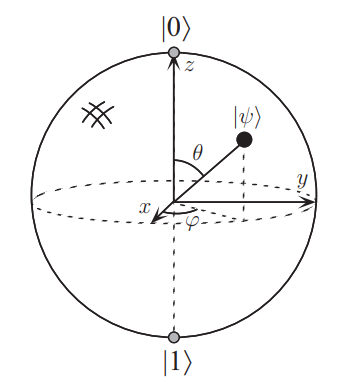
\includegraphics[scale=0.70]{imagenes/Bloch.png}
    \caption{Representación de un estado cuántico en la esfera de Bloch.
\textbf{Fuente:} Nielsen y Chuang \cite{nielsen_chuang_2011}.}
    \label{fig:Bloch}
\end{figure}
La representación de un qubit en la esfera de Bloch esta dada por la ecuación: 
\begin{equation}
    \label{ec:Bloch_rep}
    \ket{\psi} = \cos{\frac{\theta}{2}}\ket{0}+ e^{i\phi}\sin{\frac{\theta}{2}}\ket{1},
\end{equation}
con $\theta,\phi$,  ángulos que recorren la esfera (ver figura \ref{fig:Bloch}), y toman los valores:
\begin{equation}
 0 \leq \theta \leq \pi ;  \quad   0 \leq \phi \leq 2\pi.
\end{equation} 
La ecuación \ref{ec:Bloch_rep} nos permite representar estados puros en la esfera de Bloch. Sin embargo, para cualquier estado $\rho$ de un qubit, usamos el vector de Bloch, cuyas componentes señalan un punto en la esfera \cite{princip_quantum}.

Para definir el vector de Bloch transformamos los parámetros $\theta,\phi$ a coordenadas cartesianas como $\textbf{r} = (x,y,z)$ de la forma:
\begin{equation}
\left\{\begin{matrix}
x = |\textbf{r}| \sin{(\theta)} \cos{(\phi)} \\
y = |\textbf{r}| \sin{(\theta)} \sin{(\phi)} \\
z = |\textbf{r}| \cos{(\theta)}.
\end{matrix}\right. 
\end{equation}
El valor absoluto $|\textbf{r}|=1$ para estados puros, mientras que
$|\textbf{r}|<1$ para estados mixtos. Notemos que los estados puros se
encuentran en la superficie de la esfera de Bloch, mientras que los estados
mixtos en el interior. Por lo tanto, obtenemos otra representación útil de la
ecuación \ref{ec:Bloch_rep} mediante el operador $\rho$ para estados puros como
:
\begin{equation}    \label{ec:vec_bloch}
    \rho  = \frac{1}{2} ( \mathbb{1} + \textbf{r} \cdot \sigma),
\end{equation}
donde $\sigma $ es llamado el vector de Pauli, con las matrices:
\begin{equation}
\label{ec:pauli_matrix}
\sigma_x= \begin{pmatrix}
    0 & 1 \\
    1 & 0 \\
\end{pmatrix} ;\quad 
\sigma_y= \begin{pmatrix}
    0 & -i \\
    i & 0 \\
\end{pmatrix};\quad
\sigma_z= \begin{pmatrix}
    1 & 0 \\
    0 & -1 \\
\end{pmatrix}.
\end{equation}

Las compuertas cuánticas son operadores unitarios reversibles $U$ de dimensión
$n\times n $. Estas actúan linealmente sobre qubits que pueden estar en
superposición. Además, se visualizan por cajas que contienen las iniciales del
operador aplicado (ver figura \ref{fig:compuerta}). 

  \begin{figure}[h]
        \centering
        \begin{quantikz}
        \qw & \gate{U} & \qw
        \end{quantikz}
        \caption{Representación de compuerta cuántica $U$. \textbf{Fuente:} elaboración propia.     }
        \label{fig:compuerta}
    \end{figure}
    
Los operadores $U$ que actúan sobre un qubit son de dimensión $2 \times 2$, y se representan por la matriz:
\begin{equation}
    U = \begin{pmatrix}
    u_{00} & u_{01}  \\
    u_{10} & u_{11} 
    \end{pmatrix}.
\end{equation}
Nos enfocaremos en un conjunto específico de compuertas de uno y varios qubits
necesarias para este trabajo, comenzando con las compuertas de rotación en los
ejes de la esfera de Bloch: $R_x$, $R_y$ y $R_z$. Estas compuertas rotan el
estado del qubit alrededor de cada eje de la esfera de Bloch y pueden
interpretarse como versiones parametrizadas de los operadores de Pauli (ver
ecuación \ref{ec:pauli_matrix}). La representación de cada rotación es:
\begin{align}
    R_x(\theta) &=  \begin{bmatrix}
    \cos{(\theta)} & -i\sin{(\theta)}\\
    -i\sin{(\theta)} & \cos{(\theta)} 
    \end{bmatrix},  \\
    R_y(\theta) &=  \begin{bmatrix}
    \cos{(\theta)} & -\sin{(\theta)}\\
    \sin{(\theta)} & \cos{(\theta)} 
    \end{bmatrix}, \\
    R_z(\theta) &=  \begin{bmatrix}
    e^{-i\theta} & 0\\
    0 & e^{i\theta} 
    \end{bmatrix}.
\end{align}
Si aplicamos una rotación con un ángulo $\pi/2$ es equivalente a aplicar los
operadores de Pauli $X,Y,Z$. Esto cambia la dirección del estado en su
respectivo eje (ver figura \ref{fig:rep_pauli}). 

\begin{figure}[h!] % {{{
    \centering
    % Subfigura para X y Y en la misma fila
    \begin{subfigure}{0.45\textwidth}
        \centering
        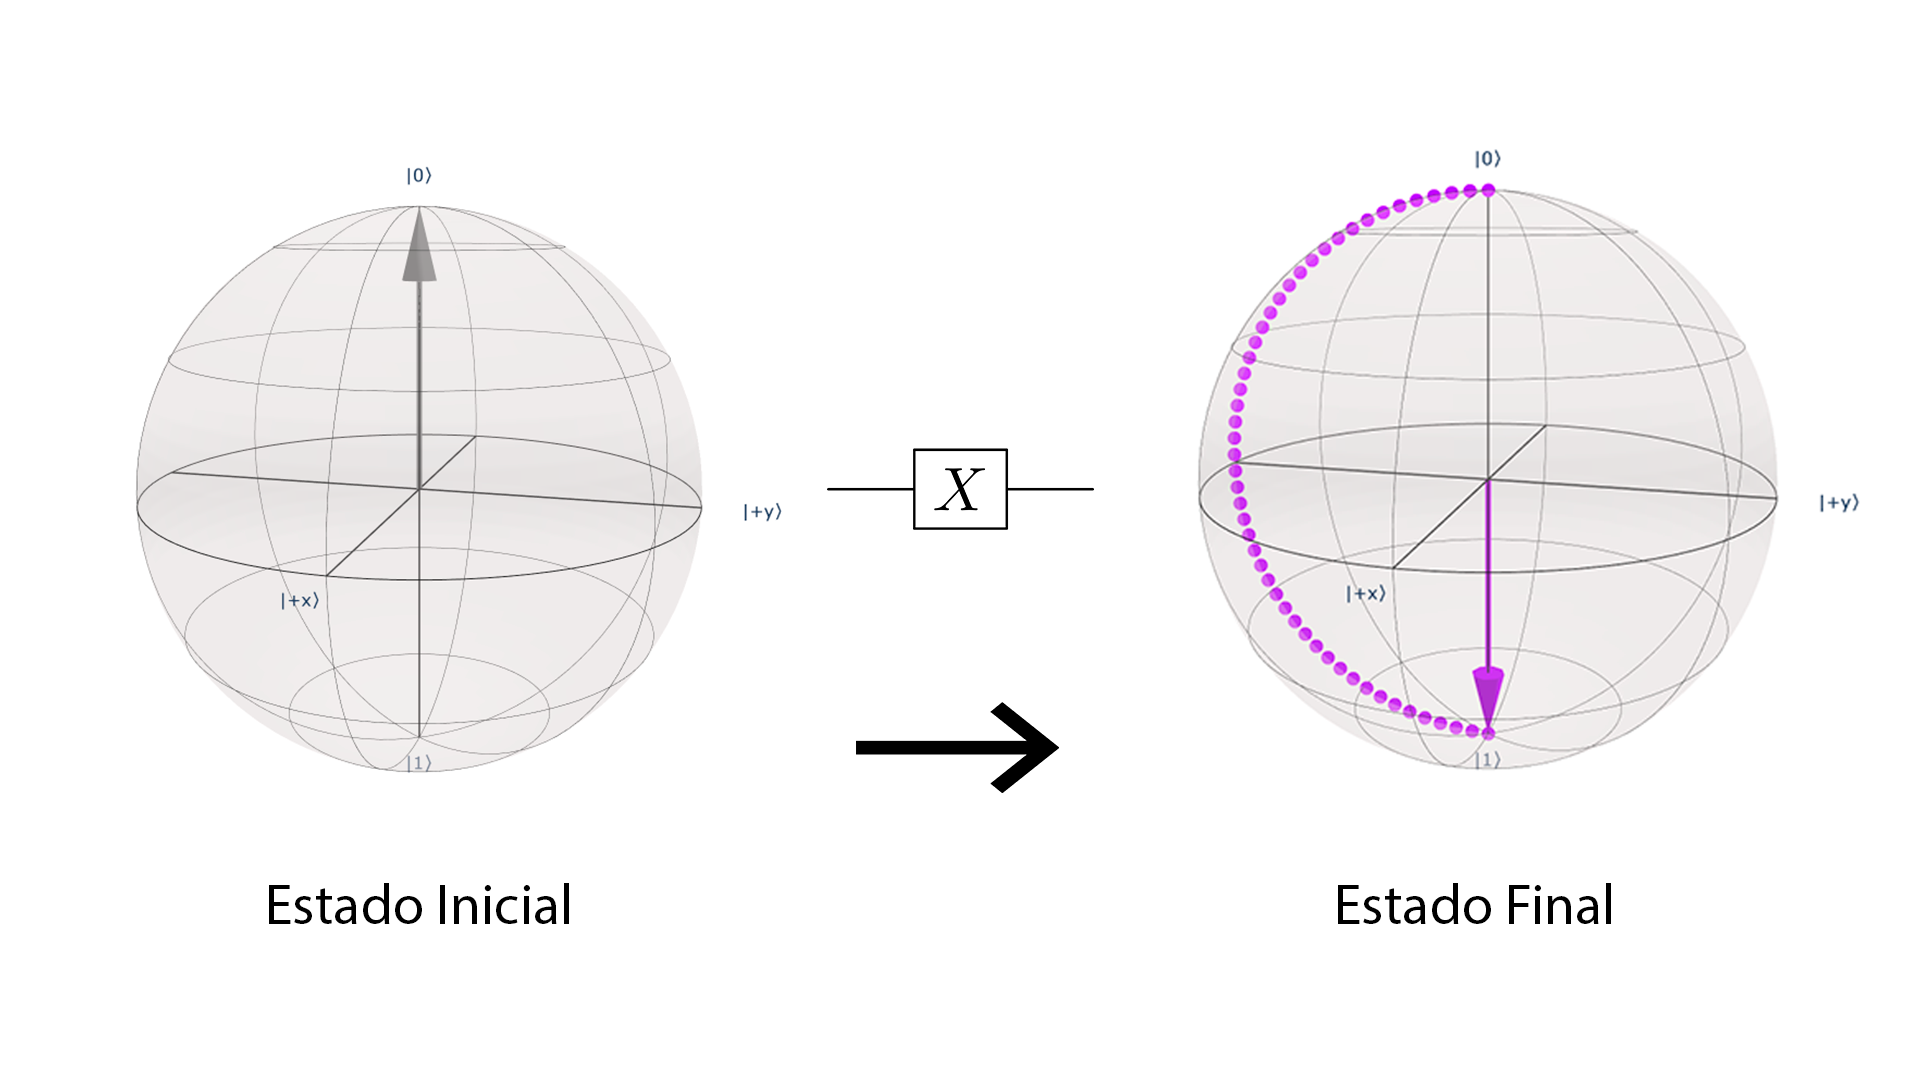
\includegraphics[width=\linewidth]{imagenes/Paulix.png}
        \caption{Representación visual de la acción de $X$ en la esfera de Bloch.}
        \label{fig:choi_p0.1}
    \end{subfigure}
    \hspace{1em} % Espacio horizontal entre las dos primeras subfiguras
    \begin{subfigure}{0.45\textwidth}
        \centering
        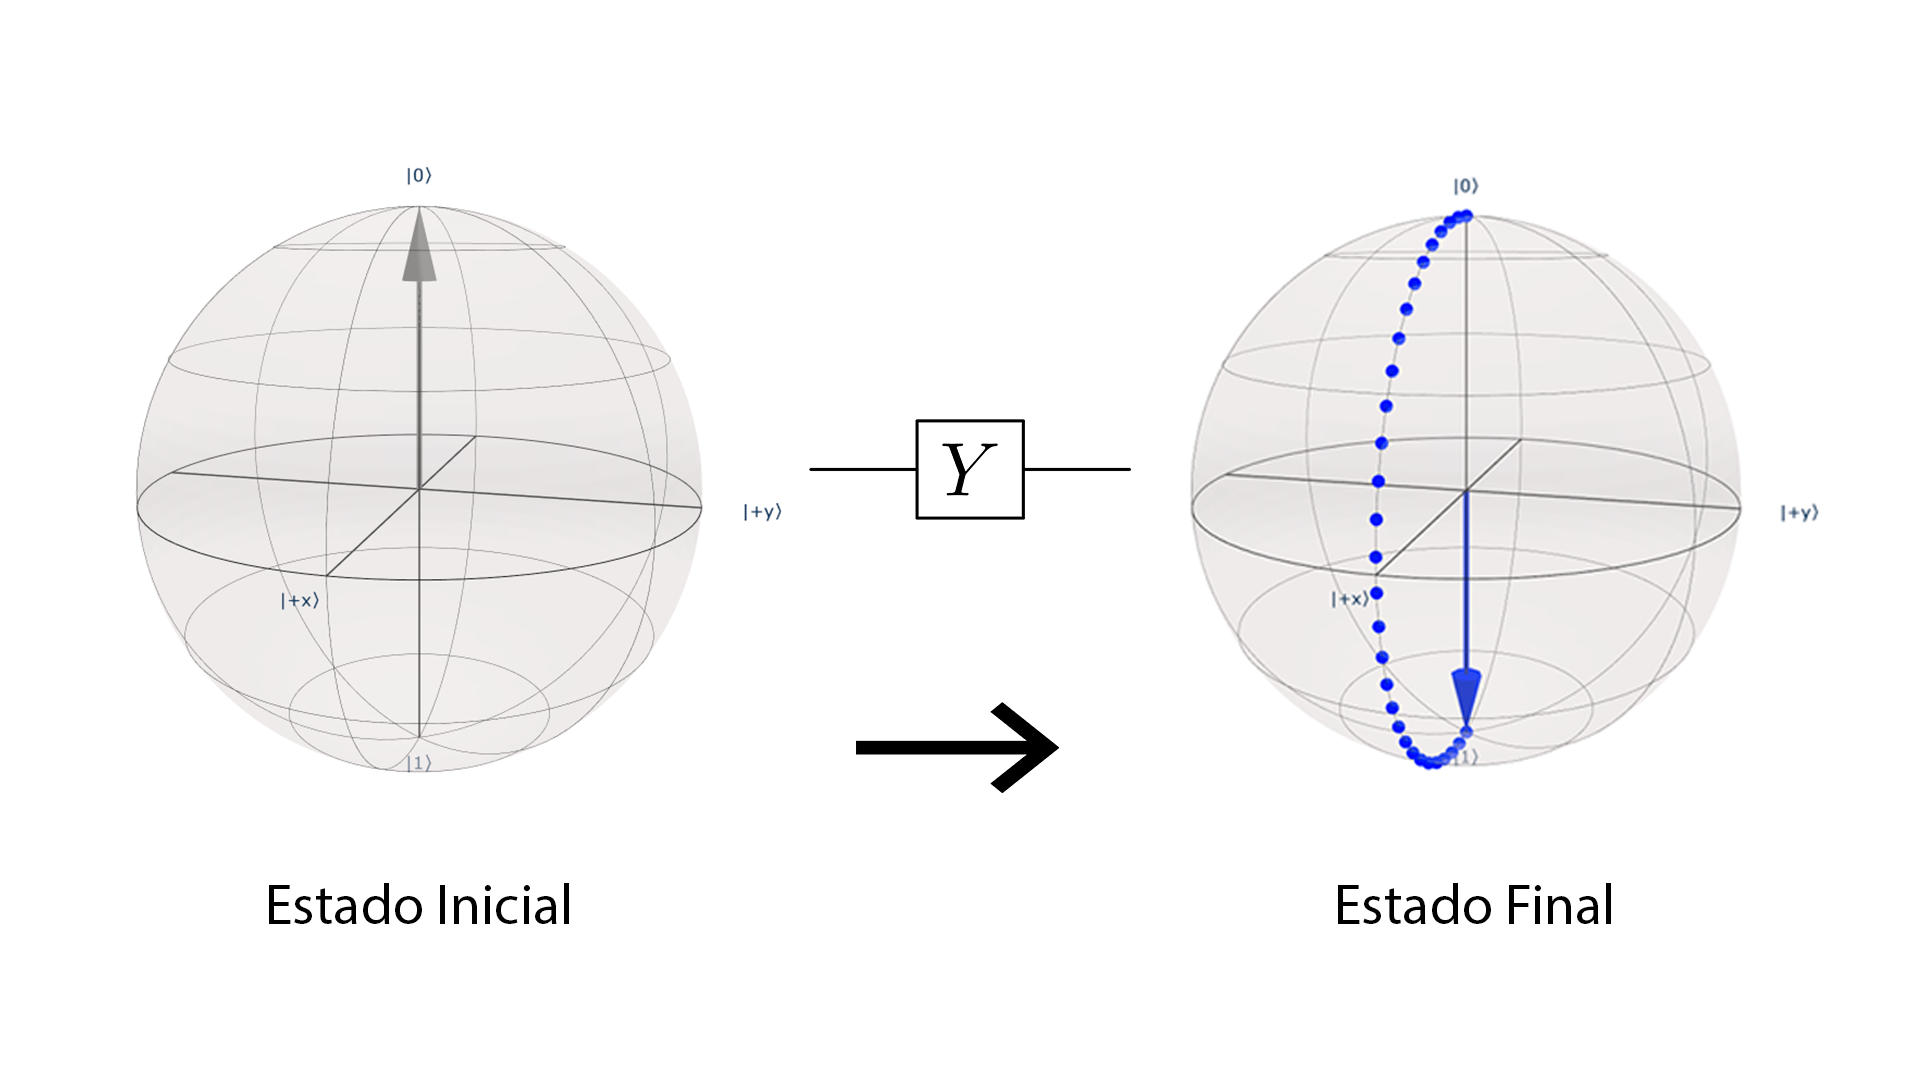
\includegraphics[width=\linewidth]{imagenes/Pauliy.png}
        \caption{Representación visual de la acción de $Y$ en la esfera de Bloch.}
        \label{fig:choi_p0.9}
    \end{subfigure}

    % Subfigura para Z en una fila inferior
    \vspace{1em} % Espacio vertical entre las filas
    \begin{subfigure}{0.45\textwidth}
        \centering
        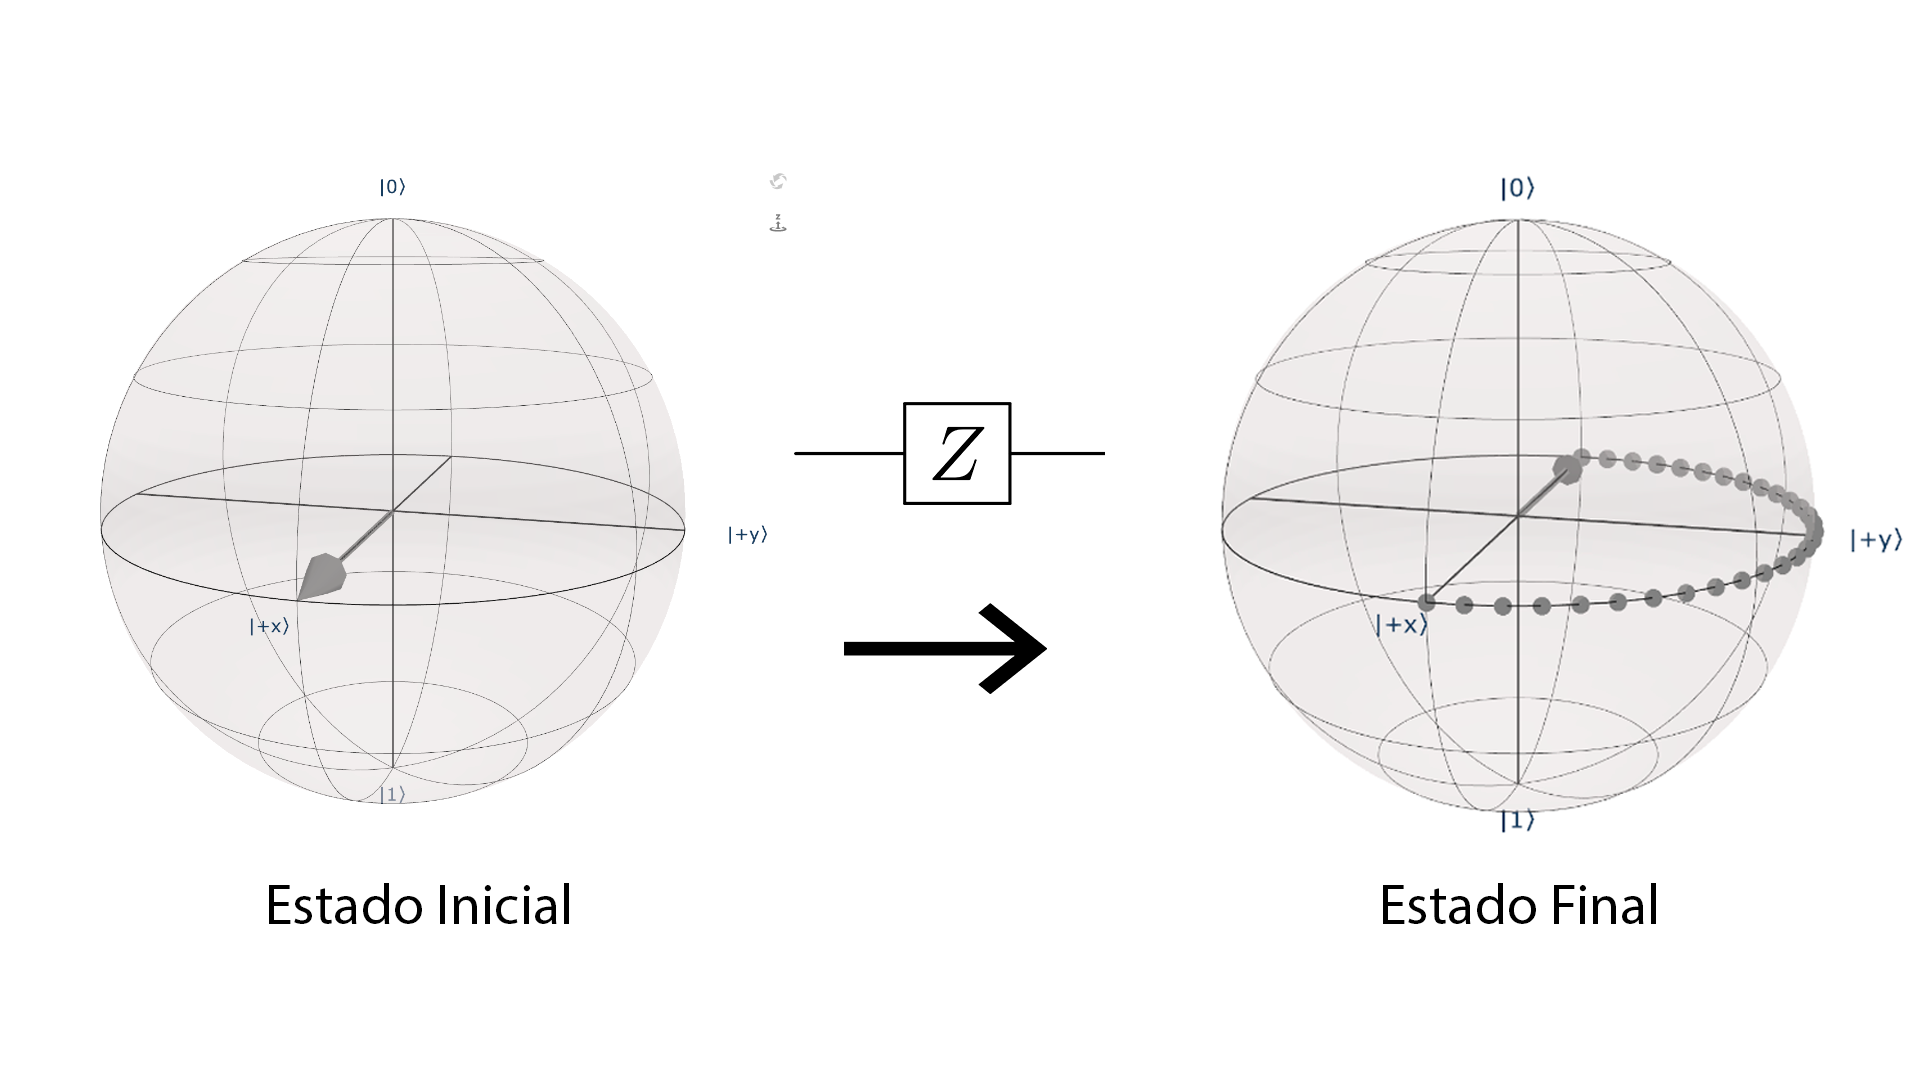
\includegraphics[width=\linewidth]{imagenes/Pauliz.png}
        \caption{Representación visual de la acción de $Z$ en la esfera de Bloch.}
        \label{fig:choi_p0.9}
    \end{subfigure}
    
    \caption{Representación visual de las compuertas de rotación en la esfera de Bloch. \textbf{Fuente:} elaboración propia}
    \label{fig:rep_pauli}
\end{figure} % }}}

Además de las compuertas de Pauli, necesitamos de una compuerta que haga otro
tipo de cambio en la base de un qubit, como lo es la compuerta de
Hadamard. Esta compuerta tiene la característica de poner en
superposición de igual amplitud a los estados de la base de un qubit.
La matriz que la describe es
\begin{equation}
    H= \frac{1}{\sqrt{2}}
    \begin{pmatrix}
     1& 1 \\
     1& -1 \\
    \end{pmatrix},
\end{equation} 
Su acción se ve como una rotación de $\pi$ radiantes sobre el eje
$(x+z)/\sqrt{2}$ en la esfera de Bloch.  También puede descomponerse como la
sucesión de $\pi$ radianes en el eje $x$, seguido de una rotación de $\pi/2$ en
$y$ (ver figura \ref{fig:hadamard}).

\begin{figure}
    \centering
    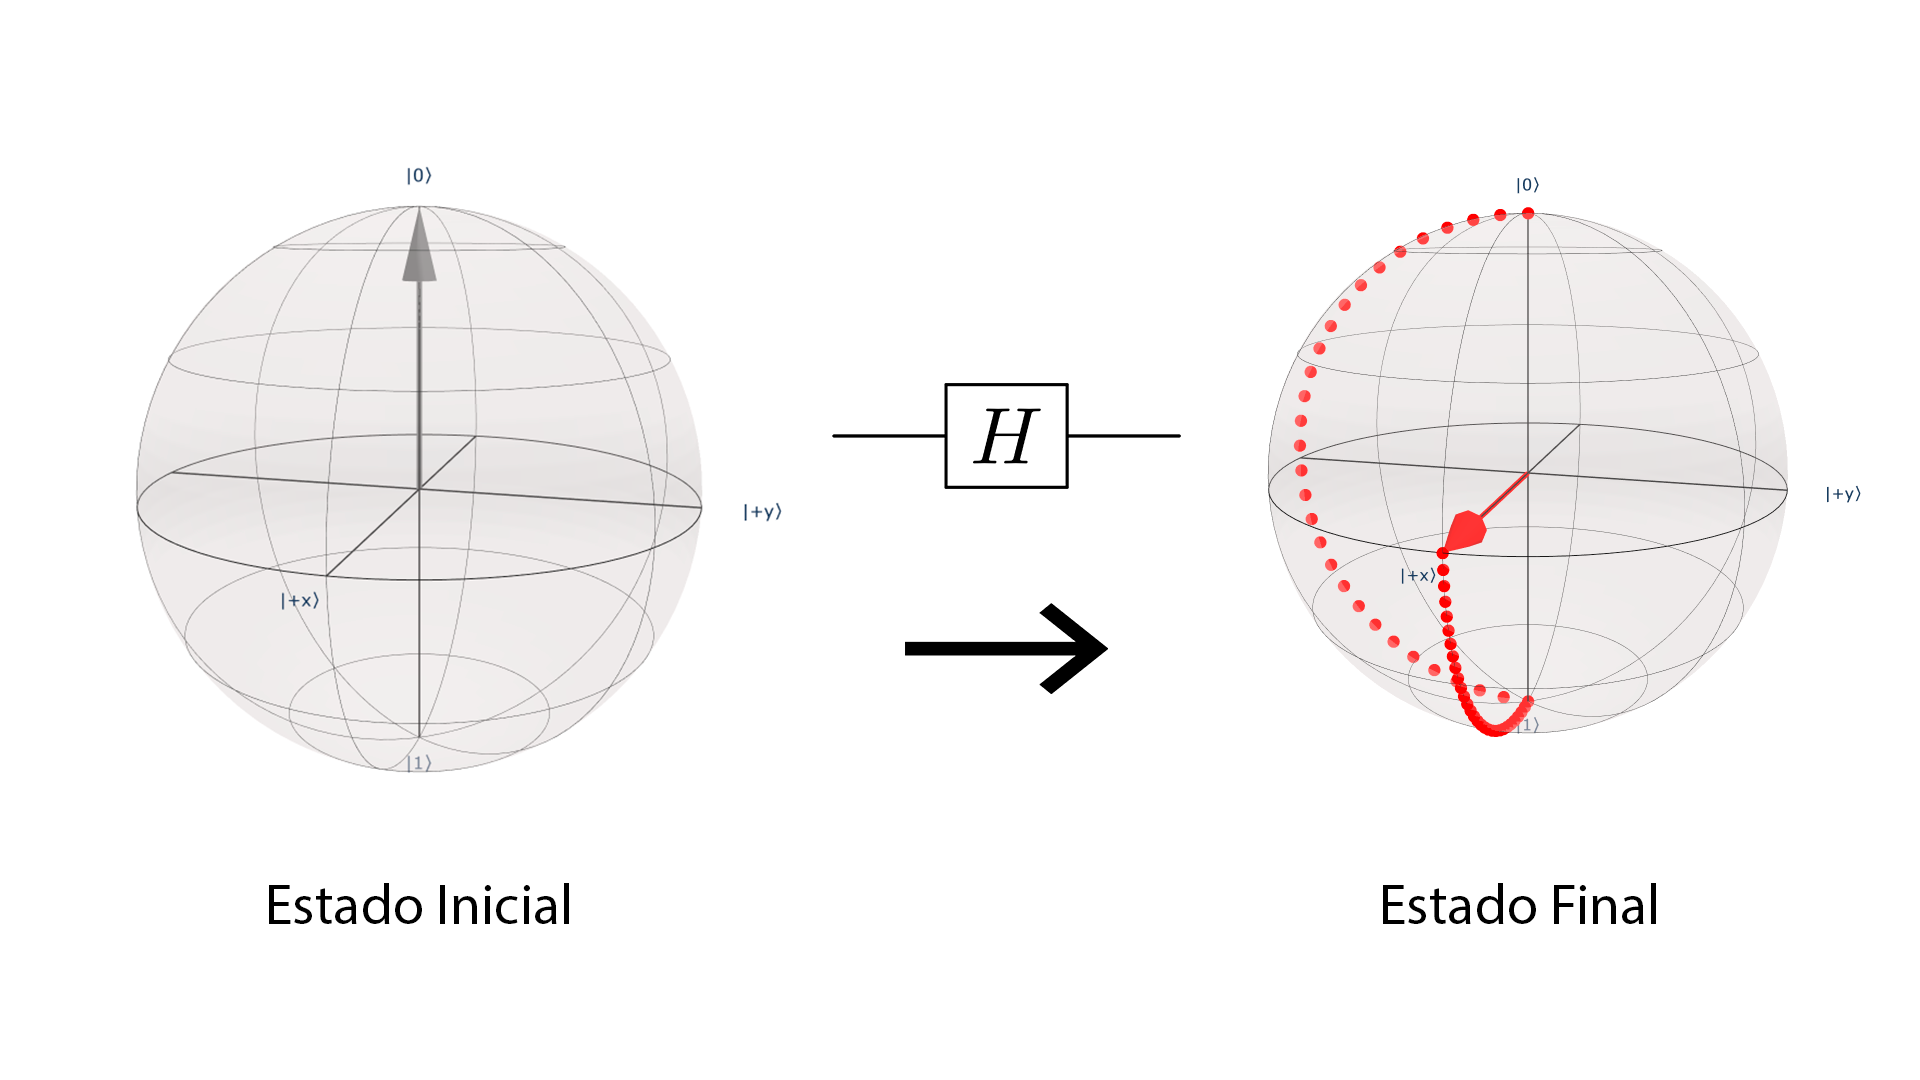
\includegraphics[scale=0.15]{imagenes/Haddamard.png}
    \caption{Representación visual de la acción de la compuerta de Hadamard sobre un estado inicial $\ket{0}$ en la esfera de Bloch.}
    \label{fig:hadamard}
\end{figure}

Las compuertas anteriores son importantes al trabajar con un qubit, sin
embargo, para trabajar con varios qubits usamos compuertas de control.
Estas compuertas hacen uso de un qubit con el rol de  control, el cual
regula la acción de otros qubits que tienen el rol de objetivo.

Las compuertas de control unitario de dos qubits $CU$, son representadas por la matriz:
\begin{equation}
    CU = 
    \begin{pmatrix}
    \label{ec:2.27}
    1 & 0 & 0 & 0 \\
    0 & 1 & 0 & 0 \\
     0& 0 & u_{00} & u_{01} \\
     0&  0&  u_{10}&u_{11} \\
    \end{pmatrix},
\end{equation}
donde $u_{ij}$ son los elementos de la compuerta unitaria $U$ que actúa sobre el qubit objetivo.

En esta matriz, el primer cuadrante es una identidad que garantiza que, si el qubit de control está en el estado $\ket{0}$, el qubit objetivo permanece sin cambios. Si el qubit de control está en $\ket{1}$, el bloque inferior derecho aplica la transformación unitaria $U$ al qubit objetivo. Esto permite implementar distintas compuertas de control, como $CR_x$ \footnote{La compuerta $CX$ es comúnmente conocida como compuerta $CNOT$. En adelante, cuando hablemos de la compuerta $CNOT$, nos referimos a $CR_x(\pi/2)$.}  o $CR_z$, ajustando los parámetros $u_{ij}$.

Al realizar una medición cuántica hace que nuestro qubit colapse a uno de los estados de la base $ \sigma_z$. Sin embargo, es posible realizar un cambio de base y poder medir en otro tipo de bases. A continuación daremos la definición de Nielsen y Chuang \cite{nielsen_chuang_2011}:

Dada cualquier base de estados $\ket{a},\ket{b}$ para un qubit, es posible expresar un estado arbitrario como una combinación lineal $\alpha\ket{a}+\beta\ket{b}$ de esos estados. Además, siempre que los estados sean ortonormales,  \textbf{es posible realizar una medición respecto a la base de $\ket{a},\ket{b}$}, dando un resultado $a$, con probabilidad $|\alpha|^2$ y $b$, con probabilidad $|\beta|^2$. 

\begin{ex}\label{Ejemplo 2.1.1} \end{ex}
 Supongamos un estado arbitrario $\ket{\psi}=\alpha \ket{0} + \beta\ket{1}$, del cual buscamos medir en una nueva base:
 \begin{align}
 \label{ec:2.32}
     \ket{+} & \equiv \frac{1}{\sqrt{2}} (\ket{0} + \ket{1}) \\
    \ket{-} & \equiv \frac{1}{\sqrt{2}} (\ket{0}-\ket{1}).
 \end{align}
Si re expresamos $\ket{\psi}$ en la nueva base veremos que:
 \begin{align}
     \ket{\psi}  &= \alpha\ket{0} + \beta\ket{1} \\
                 &= \frac{\alpha}{\sqrt{2}} ( \ket{+ } + \ket{-}) + \frac{\beta}{\sqrt{2}} (\ket{+} + \ket{-})\\
                 & = \frac{\alpha+\beta}{\sqrt{2}} \ket{+} + \frac{\alpha-\beta}{\sqrt{2}} \ket{-} . 
 \end{align}
Al medirlo en la base $\{\ket{+}, \ket{-}\}$, obtendremos probabilidades $|\alpha+\beta|^2$ y $|\alpha-\beta|^2$ respectivamente.

Las mediciones en otras bases serán de utilidad para la tomografía de estado ya que hace uso de distintas mediciones en distintas bases para recuperar la información de un estado cuántico.
% }}}
\subsection{Composición de circuitos cuánticos} % {{{

Un circuito cuántico es una rutina computacional con operadores que actúan
sobre qubits. Los circuitos se conforman por cables, compuertas y mediciones.
Un cable se usa como representación de un qubit en estado inicial $\ket{0}$.  
Como vimos en la sección anterior, las compuertas cuánticas se representan con
cajas que contienen el nombre del operador, además se posicionan en el cable del qubit que actúan. Por otro lado, las compuertas de
control se identifican con un punto para el qubit de control unido a una caja
del qubit target (ver figura \ref{fig:circuito0}).

\begin{figure}[h]
    \centering
    \begin{quantikz}
    \lstick{$\ket{0}$} & \gate{X} & \ctrl{1} & \qw  \\
    \lstick{$\ket{0}$} & \qw & \gate{R_y} & \qw 
    \end{quantikz}
    \caption{Circuito de ejemplo para crear interacción entre dos qubits. \textbf{Fuente:} elaboración propia.}
    \label{fig:circuito0}
\end{figure}


Por el lado de  la medición cuántica, se representa mediante un símbolo de
``medidor''
que colapsa el estado cuántico del qubit y almacena el resultado en
bits clásicos (ver figura \ref{fig:circuito2}). En los diagramas, una línea
simple representa a los qubits, mientras que una línea doble indica los bits
clásicos resultantes de la medición.
 
    \begin{figure}[h]
        \centering
        \begin{quantikz}
        \lstick{$\ket{\psi}$} &  \meter{} & \cw{M}
        \end{quantikz}
        \caption{Circuito cuántico representativo para una medición.}
        \label{fig:circuito2}
    \end{figure}

Al conocer la composición de circuitos cuánticos, es importante un principio
que nos permitirá implementar circuitos en computadoras cuánticas
reales\cpnote{porque necesitamos este principio para implemtnar circuitos?} \felnote{Lo uso de forma implícita cuando trazamos parcialmente el entorno. Lo quito?   }.
A continuación, usaremos el principio \cpnote{Es una definicion, o un principio?} \felnote{Corregido: es un principio}
 de Nielsen y Chuang
\cite{nielsen_chuang_2011}:
%
\begin{prin}\textbf{(Principio de medición diferida)}:  Las mediciones intermedias pueden posponerse hasta el final del circuito cuántico. Si resultados de la medición son usados en algún punto del circuito, entonces los operadores de control clásicos son reemplazados por
operadores condicionales cuánticos.   
\end{prin}
\cpnote{No recuerod donde usas eso en tu trabajo. Me lo puedes señalar?}\felnote{idem con lo anterior. Lo uso de forma implícita cuando trazamos parcialmente un circuito , consideras mejor quitarlo?    }

A menudo, las mediciones cuánticas se realizan como un paso intermedio en un
circuito cuántico, y sus resultados se utilizan para controlar de manera
condicional las compuertas cuánticas que siguen.  Este es el caso, por ejemplo,
en un circuito de teleportación cuántica (ver figura \ref{fig:telep_cuant}).
Sin embargo, estas mediciones pueden moverse al final del circuito,
reemplazando las operaciones clásicas condicionales por operaciones cuánticas
equivalentes (ver figura \ref{fig:telep_cuant_dif}).

\begin{figure}[h]
    \centering
    \begin{quantikz}
    \lstick{$\ket{\psi}$} \qw & \ctrl{1} & \gate{H} & \meter{$M_1$} & \cw & \cw & \cwbend{2} & \\
    \lstick[wires=2]{$\ket{\beta_{00}}$} \qw & \targ{} & \qw & \meter{$M_2$} & \cw & \cwbend{1} \\
    \qw & \qw & \qw & \qw & \qw & \gate{X^{M_2}} & \gate{Z^{M_1}} & \qw \rstick{$\ket{\psi}$}\\
    \end{quantikz}
    \caption{Circuito de teleportación cuántica. Las líneas dobles representan
el traslado de información en bits clásicos. El estado $\ket{\beta_{00}}$ representa un estado de Bell. \textbf{Fuente:} Nielsen y Chuang \cite{nielsen_chuang_2011}.}
    \label{fig:telep_cuant}
\end{figure}	

\begin{figure}[h]
    \centering
    \begin{quantikz}
    \lstick{$\ket{\psi}$} \qw & \ctrl{1} & \gate{H} & \qw  & \ctrl{2} & \qw  & \meter{}\\
    \lstick[wires=2]{$\ket{\beta_{00}}$} \qw & \targ{} & \qw &  \ctrl{1} & \qw & \qw & \meter{} \\
    \qw & \qw & \qw & \gate{X} & \gate{Z} & \qw & \qw       \rstick{$\ket{\psi}$}\\
    \end{quantikz}
    \caption{Circuito equivalente de teleportación, usando el principio de medición diferida. \textbf{Fuente:} Nielsen y Chuang \cite{nielsen_chuang_2011}.}
    \label{fig:telep_cuant_dif}
\end{figure}


% Desarrollaremos un principio importante para las mediciones en circuitos cuánticos: principio de medición diferida. El principio nos indica que las mediciones pueden ser llevadas siempre al final del circuito.  

% }}}
\subsection{Plataforma \textit{IBM Quantum Experience}} % {{{

Para este trabajo utilizaremos la plataforma de \textit{IBM Quantum
Experience}. Esta plataforma nos da acceso a computadoras cuánticas para
ejecutar circuitos cuánticos válidos. La conexión a las computadoras se hace
por medio de la librería de qiskit de \textit{Python}.  

Podemos correr circuitos cuánticos en la plataforma por medio de simuladores,
que emulan de forma cercana el comportamiento de una computadora cuántica, con
capacidad de hasta 5000 qubits \cpnote{dudo este numero. tienes alguna referencia?} \felnote{Quisiera que hablemos sobre esto, desde la versión 1.0 ya no aparecen los simuladores en el dashboard (https://quantum.ibm.com/services/resources), hice pruebas con las funciones actuales y no pasa de 16 qubits. Encontré cuando sí decía 5000 en el internet archive (ver quantum\_resources\_archive.png) .}. También podemos correr los circuitos en
computadoras cuánticas reales,  con capacidad de hasta 127 qubits de forma
gratuita \cite{ibm_quantum_resources}\cpnote{Checa, no se si siga siendo gratuito y no se si ese numero de 7 está 
actualizado} \felnote{Corregido: lo actualicé a 127 (https://quantum.ibm.com/services/resources) , pero también quisiera que lo hablaramos.}. En este trabajo haremos uso de los servicios gratuitos en la
plataforma.  

Al ejecutar un circuito en una computadora cuántica se pasa por un proceso llamado transpilación. Este se encarga de reescribir un circuito cuántico para que se adapte a la topología de un dispositivo cuántico específico. También optimiza sus instrucciones para su ejecución en computadoras cuánticas con presencia de ruido.(ver figura \ref{fig:transpiling}). 
\begin{figure}[h]
    \centering
    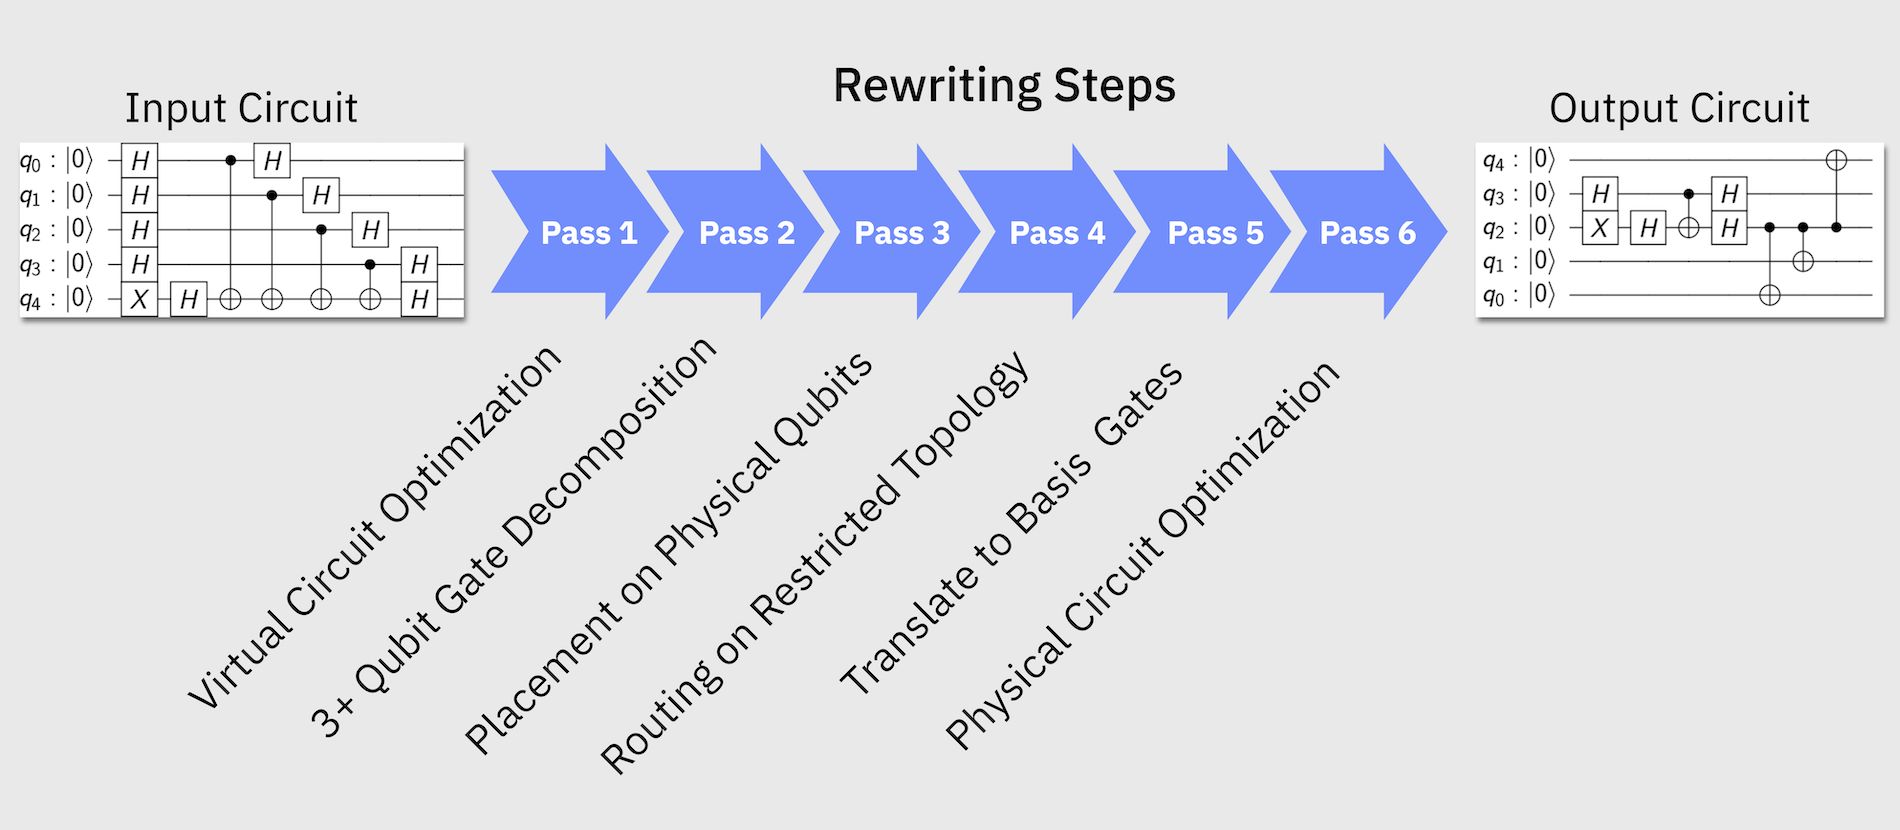
\includegraphics[scale=0.20]{imagenes/transpiling_core_steps.png}
    \caption{Proceso de transpilación para un circuito cuántico en la plataforma de IBM} \textbf{Fuente}: IBM Quantum API \cite{ibm_quantum_api}
    \label{fig:transpiling}
\end{figure}
La topología del sistema influye directamente en como se implementan las interacciones entre qubits dentro del circuito cuántico, especialmente cuando se hacen operaciones entre qubits que no estan conectados de forma uniforme (ver figura \ref{fig:topos}). 
\begin{figure}[h]
    \centering
    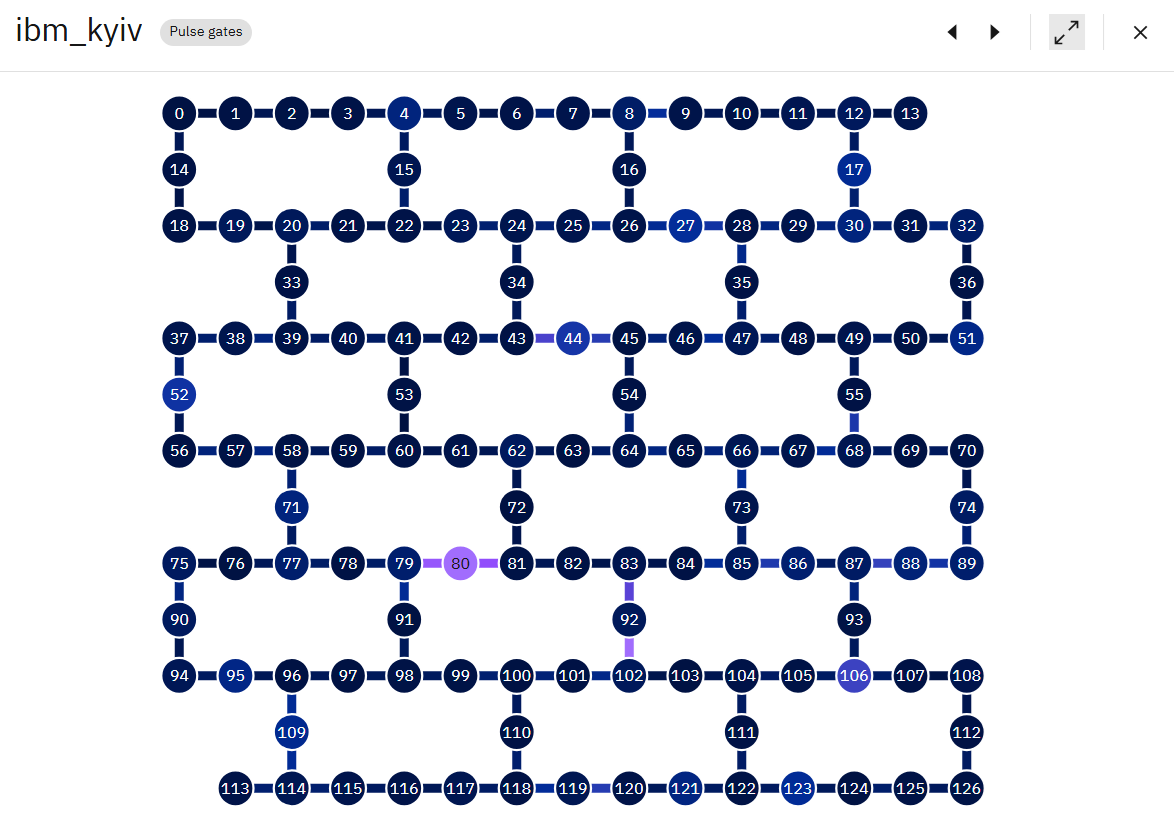
\includegraphics[scale=0.5]{imagenes/topo_ibm_kyiv.png}
    \caption{Topología correspondiente a la computadora cuántica IBM\_Kyiv de IBM, con capacidad de 127 qubits. Fuente: IBM Quantum Resources \cite{ibm_quantum_resources}}
    \label{fig:topos}
\end{figure}
\begin{ex} \label{ex:transpilation} \end{ex}
El circuito cuántico mostrado en la figura \ref{fig:circuito7}  se aplica una compuerta $Z$ al qubit $q_3$ , segudo una compuerta $CNOT$ entre los qubits $q_3$ y $q_0$. De forma similar, los qubits $q_2$ y $q_0$ interactúan a través de otra compuerta $CNOT$. Supongamos que buscamos ejecutar este circuito en la computadora cuántica con la topología de la figura \ref{fig:topos}. Ya que los qubits $q_0,q_3$ y $q_0,q_2$ no interaccionan directamente, debemos reescribir nuestro circuito para esta topología. La transpilación resultante se puede ver en la figura \ref{fig:circuito8}).  

\begin{figure}[h]
\centering
\begin{quantikz}
\lstick{$q_0$} & \qw      & \ctrl{3} & \ctrl{2} & \qw \\
\lstick{$q_1$} & \qw      & \qw      & \qw      & \qw \\
\lstick{$q_2$} & \qw      & \qw      & \targ{}  & \qw \\
\lstick{$q_3$} & \gate{Z} & \targ{}  & \qw      & \qw
\end{quantikz}
\caption{Circuito inicial correspondiente al ejemplo \ref{ex:transpilation}. \textbf{Fuente:} elaboración propia.}
\label{fig:circuito7}
\end{figure}


\begin{figure}[h]
\centering
\begin{quantikz}
\lstick{$q_0$} & \qw      & \qw & \qw & \qw & \qw & \qw \\
\lstick{$q_1$} & \gate{H} & \qw      & \qw      & \ctrl{1}  & \gate{H} & \qw\\
\lstick{$q_2$} & \qw      & \ctrl{1}     & \gate{H}  & \targ{} & \gate{H} & \qw\\
\lstick{$q_3$} & \gate{Z} & \targ{}  & \qw      & \qw & \qw & \qw
\end{quantikz}
\caption{Circuito final correspondiente al ejemplo \ref{ex:transpilation}, luego de ser transpilado. \textbf{Fuente:} elaboración propia.}
\label{fig:circuito8}
\end{figure}
La transpilación de circuitos viene incorporada en la librería de Qiskit, es necesaria para ejecutar circuitos en computadoras cuánticas reales y será un componente clave del proyecto. Invitamos al lector a indagar más a detalle en la documentación de la librería \cite{qiskit_transpiler}.


%=================================================




% }}}
% }}}
\section{Canales Cuánticos y su representación} % {{{
Una forma natural de describir la dinámica de un sistema cuántico abierto es considerar que este surge de la interacción de un sistema de interés , al que llamaremos sitema principal , y un \textit{entorno}, que juntos forman un sistema cuántico cerrado \cite{nielsen_chuang_2011}:
\begin{equation}\label{ec:rep_sist_abierto}
    \rho = \rho_{\text{sp}} \otimes \rho_{\text{ent}}.
\end{equation}
Supondremos que la interacción entre ambos sistemas se da por una transformación unitaria $U$, luego de esto, el sistema ya no interactúa con el entorno resultando en el estado final del sistema pincipal $\mathcal{E}$:
\begin{equation}
    \mathcal{E}(\rho_{\text{sp}}) = \text{Tr}_{\text{ent}}[ U( \rho_{\text{sp}} \otimes \rho_{\text{ent}} ) U^\dagger ].
\end{equation}
Notemos que si $U$ no involucra ninguna interacción entre el sistema y el entorno entonces  $\mathcal{E}(\rho_{sp}) =  \widetilde{U} \rho \widetilde{U}^\dagger \footnotemark$\footnotetext{A partir de los siguientes enunciados se utilizará $\rho = \rho_{\text{sp}}$ ya que se entiende de forma implícita que nos referimos a $\rho$ como el sistema principal.} , donde $\widetilde{U}$ es la parte de $U$ que interactúa solo con el sistema principal. Este proceso describe cómo los operadores de evolución de sistemas cuánticos cerrados pueden ser generalizados a operadores cuánticos $\mathcal{E}$ (también conocidos como superoperadores), que mapean matrices de densidad del sistema a nuevos estados cuánticos, teniendo en cuenta las influencias del entorno.

Los operadores cuánticos pueden ser representados de forma explícita en términos del espacio de Hilbert de los operadores del sistema principal. Donde $\ket{e_k}$ es una base ortonormal del espacio del entorno, y $\rho_{ent} = \ketbra{e_0}$ su estado inicial, asumimos que:
\begin{align}
\mathcal{E}(\rho) &= \text{Tr}_{\text{ent}}[ U( \rho \otimes \ketbra{e_0} ) U^\dagger ] \\
&= \sum_k E_k \rho E_k^\dagger.  \label{ec:Canal_Kraus}
\end{align}
En esta expresión, cada operador $E_k \equiv \bra{e_k} U \ket{e_0}$ actúa sobre el espacio del sistema principal. Esta formulación es conocida como la representación de Kraus de $\mathcal{E}$. Los operadores $\{E_k\}$ son denominados peradores de Kraus. Además, esta representación caracteriza a $\mathcal{E}$ como un operador completamente positivo (CP).

Los operadores $\{E_k\}$  satisfacen la relación de completitud, que requiere que la traza de $\mathcal{E}(\rho) = 1$:
\begin{align}
    \text{Tr}(\mathcal{E}(\rho)) &= \text{Tr}\left(\sum_k E_k \rho E_k^\dagger\right) \\
    &= \text{Tr}\left(\rho \sum_k E_k^\dagger E_k \right).
\end{align}
Notemos que para que esto se cumpla entonces:
\begin{equation}
    \sum_k E_k^\dagger E_k = I. \label{ec:trace_preserving}
\end{equation}
Esta propiedad caracteriza a los operadores $\mathcal{E}$ que preservan la traza (TP). Por lo tanto, decimos que un canal cuántico $\mathcal{E}$ es un operador completamente positivo y  que preserva la traza (CPTP), cumpliendo con las ecuaciones \ref{ec:Canal_Kraus}  y\ref{ec:trace_preserving}. 

Mientras que la representación de Kraus ofrece una forma de describir los canales cuánticos, la matriz de Choi proporciona una representación alternativa útil para su caracterización. 
La matriz de Choi de un canal cuántico $\mathcal{E}$ se define como \cite{QProcess}:
\begin{equation} 
\Lambda_{\mathcal{E}} = (I \otimes \mathcal{E})(|\Omega\rangle\langle\Omega|),
\end{equation} 
donde $\ket{\Omega}$ es un estado máximamente entrelazado no normalizado $\ket{\Omega} = \sum_i \ket{ii}$ .
Desarrollando el el término $|\Omega\rangle\langle\Omega|$ obtenemos:
\begin{equation}
|\Omega\rangle\langle\Omega| = \sum_{i,j=1}^{d} \ketbra{i}{j} \otimes \ketbra{i}{j},
\end{equation} 
que nos deja la segunda representación de la matriz de Choi
\cite{Qiskit_documentation} \cite{QProcess}:
\begin{equation}\label{ec:Choi_ketbra}
\Lambda_{\mathcal{E}} = \sum_{i,j=1}^{d} \ketbra{i}{j} \otimes \mathcal{E}(\ketbra{i}{j}).
\end{equation}
Esta expresión representa la superposición de todas las posibles transformaciones que $\mathcal{E}$ puede aplicar sobre la base computacional del sistema principal luego de su interacción con el entorno. Esto permite ver el efecto del canal sobre cualquier estado del sistema principal.


La matriz de Choi tiene  varias propiedades descritas en el paper de  G. Homa  y otros \cite{Choi2024},  que permiten describir completamente un canal cuántico y hacer una correlación con la representación de Kraus:
\begin{enumerate}
     \item Para un operador $\mathcal{E}$ completamente positivo, dado en una representación de Kraus, su matriz de Choi es \textit{Hermítica}, es decir $\Lambda_{\mathcal{E}} = \Lambda_{\mathcal{E}}^{\dagger}$.\\ 
        La transpuesta conjuntada de la matriz de Choi es: 
        \begin{equation*}
            \Lambda_{\mathcal{E}}^\dagger = \left( \sum_{i,j} \ketbra{i}{j} \otimes \mathcal{E}(\ketbra{i}{j}) \right)^\dagger.
        \end{equation*}
        Utilizando la propiedad de la transpuesta conjuntada $(A \otimes B)^\dagger = A^\dagger \otimes B^\dagger$, obtenemos:
        \begin{equation}
          \Lambda_{\mathcal{E}}^\dagger = \sum_{i,j} (\ketbra{i}{j})^\dagger \otimes \mathcal{E}(\ketbra{i}{j})^\dagger.  
        \end{equation}
        Sabemos que $(\ketbra{i}{j})^\dagger = \ketbra{j}{i}$ y que $\mathcal{E}(\ketbra{i}{j})^\dagger = \mathcal{E}(\ketbra{j}{i})$ porque $\mathcal{E}$ es un operador CP. Así, tenemos:
        \begin{equation}
         \Lambda_{\mathcal{E}}^\dagger = \sum_{i,j} \ketbra{j}{i} \otimes \mathcal{E}(\ketbra{j}{i}).   
        \end{equation}
        Cambiando los índices de suma, podemos renombrar $i$ como $j$ y $j$ como $i$:
        \begin{equation}
           \Lambda_{\mathcal{E}}^\dagger = \sum_{j,i} \ketbra{i}{j} \otimes \mathcal{E}(\ketbra{i}{j}) = \Lambda_{\mathcal{E}}. \blacksquare
        \end{equation}
    \item Para un operador $\mathcal{E}$ completamente positivo, podemos escribirlo en términos de la matriz de Choi como:
            \begin{equation}\label{ec:canal_choi_form}
            \mathcal{E} (\rho) = \text{Tr}_1 [ \Lambda ( \rho^{T} \otimes I)] .
            \end{equation}
            Para demostrar esta expresión partimos de escribir a  $\rho$ en la base computacional:
        \begin{equation} \label{ec:densidad_computacional}
            \rho = \sum_{k,l} \rho_{k,l} \ketbra{k}{l},
        \end{equation}
        entonces:
        \begin{equation}
            \rho^{T} \otimes I = \sum_{k,l} \rho_{k,l} \ketbra{l}{k} \otimes I.
        \end{equation}
        Multiplicamos $\Lambda$ con $\rho^{T} \otimes I$:
        \begin{align}
            \Lambda(\rho^{T} \otimes I) & = \left( \sum_{i,j} \ketbra{i}{j} \otimes \mathcal{E}(\ketbra{i}{j}) \right) \left( \sum_{k,l} \rho_{k,l} \ketbra{l}{k} \otimes I \right) \\
            & = \sum_{i,j,k,l} \rho_{k,l} (  \ketbra{i}{j} ) (\ketbra{l}{k}) \otimes \mathcal{E} (\ketbra{i}{j})\\
            & =  \sum_{i,j,k,l} \rho_{k,l} \delta_{j,l} \ketbra{i}{k} \otimes \mathcal{E}( \ketbra{i}{j})\\
            & = \sum_{i,k,l} \rho_{k,l} \ketbra{i}{k} \otimes \mathcal{E}( \ketbra{i}{l}).
        \end{align}
        Si trazamos parcialmente el primer subsistema tenemos la expresión: 
        \begin{equation}
            \text{Tr}_1 [ \Lambda ( \rho^{T} \otimes I)]  = \text{Tr}_1 \left[  \sum_{i,k,l} \rho_{k,l}\ketbra{i}{k} \otimes \mathcal{E}(\ketbra{i}{l})\right],
        \end{equation}
        consideramos solo los términos donde $i=k$:
        \begin{equation}
            \text{Tr}_1 [ \Lambda ( \rho^{T} \otimes I)]  = \sum_{i,l}\rho_{i,l} \mathcal{E}(\ketbra{i}{l}) = \mathcal{E}(\rho) .\blacksquare
        \end{equation}
        Notemos también  que podemos reescribir esta expresión en términos de los operadores de Kraus:
        \begin{equation}
            \mathcal{E}(\rho) = \sum_{i,l} \rho_{i,l} \sum_k E_k \ketbra{i}{l}E_k^{\dagger},
        \end{equation}
        ya que $\rho_{i,l}$ es un escalar, y recordando la ecuación \ref{ec:densidad_computacional}, reordenamos la expresión: 
        \begin{align}
            \mathcal{E}(\rho)& = \sum_k E_k \left( \sum_{i,l}\rho_{i,l}\ketbra{i}{l}\right) E_k^{\dagger}\\
            & = \sum_k E_k \rho E_k^{\dagger}.
        \end{align}


        
    \item La matriz de Choi $\Lambda_{\mathcal{E}}$ de un mapeo completamente positivo (CP), es positivo semidefinido (no negativo).\\ 
     Tomemos cualquier estado $\ket{\psi}$:
    \begin{equation}
    \bra{\psi} \Lambda_{\mathcal{E}} \ket{\psi} = \bra{\psi} (\mathcal{I} \otimes \mathcal{E})(\ketbra{\Omega}) \ket{\psi}.
    \end{equation}
    
    Si escribimos a $\ket{\psi} = \sum_i c_i \ket{i} \otimes \ket{\psi_i}$, tenemos:
    \begin{equation}
    \bra{\psi} \Lambda_{\mathcal{E}} \ket{\psi} = \sum_{i,j} \overline{c_i} c_j \bra{\psi_i} \mathcal{E}\ketbra{i}{j}) \ket{\psi_j}.
    \end{equation}
    Debido a que $\mathcal{E}$ es completamente positivo, entonces $\mathcal{E}(\ketbra{i}{j})$ es un operador positivo semidefinido. Por lo tanto: 
    \begin{equation}
    \bra{\psi_i} \mathcal{E}(\ketbra{i}{j}) \ket{\psi_j} \geq 0,
    \end{equation}
    que sumando sobre todos los índices $i$ y $j$, obtenemos que
    \begin{equation}
    \bra{\psi} \Lambda_{\mathcal{E}} \ket{\psi} \geq 0. \blacksquare
    \end{equation}
    \item Sea $\Lambda \geq0$ una matriz hermitica de dimensión $d \times d$. Es la representación de Choi de un de un mapeo que preserva la traza (TP) sí y solo sí 
    \begin{equation}
        \text{Tr}_2 (\Lambda) = I.
    \end{equation}
    \textbf{Ida:} suponemos que $\mathcal{F}$ es un mapeo que preserva la traza. Por lo que si trazamos parcialmente el segundo subsistema tenemos:
    \begin{equation}
        \text{Tr}_2(\Lambda) = \sum_{i,j}\ketbra{i}{j}\text{Tr}( \mathcal{F}(\ketbra{i}{j})),
    \end{equation}
    ya que $\mathcal{F}$ preserva la traza, entonces $\text{Tr}( \mathcal{F}(\ketbra{i}{j})) = Tr(\ketbra{i}{j})$, por lo tanto:
    \begin{equation}
         \text{Tr}_2(\Lambda) = \sum_{i,j}\ketbra{i}{j} \delta_{ij}= \sum_i \ketbra{i}= I. 
    \end{equation}
    
    \textbf{Vuelta:} suponemos que $\text{Tr}_2(\Lambda) = I$ para $\Lambda$. Por lo que si usamos la representación del mapeo $\mathcal{F}$ según la ecuación \ref{ec:canal_choi_form} tenemos:
    \begin{align}
        \text{Tr} (\mathcal{F}(\rho)) &= \text{Tr}( \text{Tr}_1 [ \Lambda ( \rho^{T} \otimes I)]).
    \end{align}
    Usando la propiedad cíclica de la traza $\text{Tr}(AB) = \text{Tr}(BA)$:
    \begin{align}
        &= \text{Tr}[(\rho^T \otimes I) \Lambda], \\
        &= \text{Tr}[\rho^T \cdot \text{Tr}_2(\Lambda)]\\
        &= \text{Tr}(\rho^T)\\
        &=\text{Tr}(\rho).
    \end{align}
    Por lo tanto, vemos que $\text{Tr}(\mathcal{F}(\rho))= \text{Tr}(\rho)$, esto muestra que $\mathcal{F}$ preserva la traza $\blacksquare$.

    \item La matriz de Choi $\Lambda_{\mathcal{E}}$ de un operador cuántico completamente positivo y que preserva la traza (CPTP)  es única. \\
    Supongamos dos operadores distintos $\mathcal{F}$ y $\mathcal{G}$ con la misma matriz de Choi:
    \begin{equation}
       \sum_{i,j=1}^{d} \ketbra{i}{j} \otimes \mathcal{F}(\ketbra{i}{j}) =  \sum_{i,j=1}^{d} \ketbra{i}{j} \otimes \mathcal{G}(\ketbra{i}{j}).
    \end{equation}
    Esto implica que para cada par $i, j$, se debe cumplir que $\mathcal{F}(\ketbra{i}{j}) = \mathcal{G}(\ketbra{i}{j})$. Dado que los elementos $\ketbra{i}{j}$ abarcan toda la base del espacio de operadores, implica que $\mathcal{F} = \mathcal{G}$ para todos los posibles estados en el espacio $\blacksquare$.
\end{enumerate}

Tras demostrar estas propiedades, notemos  que podemos analizar si un operador $\mathcal{E}$ es CPTP al igual que con los operadores de Kraus. Sin embargo hay una diferencia fundamental entre ambas representaciones: la representación de Kraus \textit{no es única} para un canal cuántico $\mathcal{E}$.
Esta demostración se da por el Teorema 8.1 en Nielsen y Chuang \cite{nielsen_chuang_2011}:

\begin{thm}\textbf{(Teorema de libertad unitaria en la representación de Kraus):}  Supongamos dos conjuntos de operadores de Kraus $\{E_i, \ldots, E_m\}$ y $\{F_1, \ldots, F_r\}$ que representan el mismo canal cuántico. Podemos asegurar que $m = n$ añadiendo ceros a la lista más corta de operadores. Entonces, $\{E_i\}$ y $\{F_j\}$ describen el mismo canal cuántico si y solo si existe una matriz unitaria $U$ tal que $E_i = \sum_j u_{ij} F_j$, donde $u_{ij}$ es un elemento de la matriz unitaria $U$.
\end{thm}

Para probar este teorema partimos sabiendo que  $\{E_i\}$ y $\{F_j\}$ son conjuntos de operadores de Kraus para el mismo canal cuántico, tenemos que:
\begin{equation}
   \sum_i E_i^\dagger E_i = \sum_j F_j^\dagger F_j. 
\end{equation}
Definimos los estados $\ket{e_i} = E_i \ket{k}$ , $\ket{f_j} = F_j \ket{k}$. Por la definición de un operador de Kraus, podemos escribir:
\begin{equation}
  \ket{e_i} = \sum_j u_{ij} \ket{f_j},  
\end{equation} 
donde $u_{ij}$ son los elementos de una matriz unitaria $U$.\\
Por otro lado, cualquier estado $\ket{\psi}$ puede expresarse en términos de $\ket{e_i}$ y $\ket{f_j}$ de la siguiente forma:
\begin{equation}
E_i \ket{\psi} = \sum_j u_{ij} F_j \ket{\psi}.
\end{equation}
Esto demuestra que $E_i$ puede ser expresado como una combinación lineal de $\{F_j\}$ con coeficientes unitarios, mostrando que la representación de Kraus no es única y depende de la elección de la matriz unitaria $U$.\\
Por lo tanto, en adelante utilizaremos la notación de la matriz de Choi, ya que nos será de utilidad para la reconstrucción de canales cuánticos en la tomografía de proceso y la fidelidad de proceso al ejecutarlo en computadoras cuánticas.

\begin{ex} \label{Ejemplo 1.0.1} 
\end{ex}
El canal despolarizante  (DP, por sus siglas en inglés de Depolarizing Channel)  es un canal cuántico que introduce ruido aleatorio en un sistema, transformando cualquier estado cuántico de entrada en un estado mixto \cite{nielsen_chuang_2011}. La acción del canal actúa por una probabilidad $p$ de despolarizar un estado cuántico $\rho$ se describe de la forma:
\begin{equation} \label{ec:superop_depolarizing}
\mathcal{E}(\rho) = \text{Tr}(\rho) p  \frac{I}{2}   + (1 - p)\rho ,
\end{equation}
donde $I$ es la matriz identidad y $p$ la probabilidad mencionada. Este canal, por tanto, transforma el estado $\rho$ en una mezcla de $\rho$ y la matriz identidad, reduciendo la pureza del estado inicial. \footnote{La traza de $\rho$ convencionalmente no se muestra en textos como Nielsen y Chuang, sin embargo,  se incluye para asegurar que el canal sea CPTP.}\\
Dado que el canal  convierte cualquier estado $\rho$ en una mezcla, la acción de $\mathcal{E}$ sobre $\ketbra{i}{j}$ puede escribirse como:
\begin{equation}
\mathcal{E}(\ketbra{i}{j}) = \text{Tr}(\ketbra{i}{j})  p \frac{I}{2}+ (1 - p) \ketbra{i}{j}.
\end{equation}
Por lo que podemos ver su acción en los estados de la base:
\begin{alignat*}{2}
     \mathcal{E}( \ketbra{0}) = & (1 - \frac{p}{2} ) \ketbra{0} + \frac{p}{2} \ketbra{1}, \\
     \mathcal{E}( \ketbra{0}{1}) = & (1 - p ) \ketbra{0}{1},\\
      \mathcal{E}( \ketbra{1}{0}) = & (1 - p ) \ketbra{1}{0},\\
           \mathcal{E}( \ketbra{1}) = & (1 - \frac{p}{2} ) \ketbra{1} + \frac{p}{2} \ketbra{0}.
\end{alignat*}
Recordando la ecuación \ref{ec:Choi_ketbra}, escribimos su matriz de Choi:
% \begin{equation}
% \Lambda_{\mathcal{E}} = \frac{1}{2} \sum_{i,j=0}^{1} \ketbra{i}{j} \otimes \left(  \text{Tr}(\ketbra{i}{j} ) p  \frac{I}{2} +  (1-p) \ketbra{i}{j}  \right).
% \end{equation}
% que consiguientemente nos da la matriz 
\begin{equation}\label{ec:choi_depolarizing}
    \Lambda_\mathcal{E} = 
\begin{pmatrix}
1 - \frac{p}{2} & 0 & 0 & 1 - p \\
0 & \frac{p}{2} & 0 & 0 \\
0 & 0 & \frac{p}{2} & 0 \\
1 - p & 0 & 0 & 1 - \frac{p}{2}
\end{pmatrix}.
\end{equation}
Notemos cómo $\Lambda_{\mathcal{E}}$ refleja el funcionamiento del canal despolarizante: las entradas diagonales muestran cómo el canal mezcla el estado original con la matriz identidad, dependiendo de $p$, reduciendo la pureza del estado. Las entradas no diagonales indican las coherencias introducidas por el canal. Así, $\Lambda_{\mathcal{E}}$  nos proporciona una representación completa del efecto del canal despolarizante sobre la base computacional.  

Los canales cuánticos representarán un papel al implementarse en computadoras cuánticas. En los siguientes capítulos se detallará el proceso para implementar su matriz de Choi y reconstruirla en sistemas cuánticos.

\subsection{Tomografía y Fidelidad de Proceso Cuántico} % {{{
La tomografía de proceso cuántico (QPT) es una técnica fundamental para reconstruir experimentalmente un canal cuántico por medio de mediciones. Sin embargo, antes de hablar de la tomografía es necesario conocer la tomografía de estado cuántico.  

La tomografía de estado cuántico es un proceso para reconstruir
experimentalmente un estado desconocido a partir de un conjunto de mediciones
\cite{nielsen_chuang_2011}. El problema básico es que no existe medición
cuántica que pueda distinguir entre estados como $\ket{0}$ y
$(\ket{0}+\ket{1})/\sqrt{2}$ con certeza. No obstante, es posible estimar
$\rho$ si tenemos un gran número de copias de $\rho$. Mencionaremos el proceso
indicado en el libro de Nielsen y Chuang \cite{nielsen_chuang_2011}. 


Consideremos un estado $\rho$ y los operadores $\{\frac{\mathcal{I}}{\sqrt{2}}
\frac{X}{\sqrt{2}},  \frac{Y}{\sqrt{2}},  \frac{Z}{\sqrt{2}} \} $ que forman un
conjunto ortonormal de matrices con su respectivo producto interno. Entonces,
$\rho$ se expande como:
\begin{equation}
\label{eq:tomo_estado}
    \rho = \frac{\text{Tr}(\rho)\mathcal{I} + \text{Tr}(X\rho)X  + \text{Tr}(Y\rho)Y + \text{Tr}(Z\rho)Z}  {2}.
\end{equation}
La expresión $\text{Tr}(A\rho)$ se interpreta como el valor medio de los observables. Para esta estimación, si medimos un observable $A$ una gran cantidad de veces, $m$, obteniendo resultados $z_i$ iguales a $\pm 1$, nuestro promedio empírico de resultados sería:
\begin{equation}
    \text{Tr}(A \rho) \approx \sum_i \frac{z_i}{m}.
\end{equation}
De esta forma podemos reconstruir la matriz $\rho$ como en la ecuación \ref{eq:tomo_estado}.  

Generalizando este procedimiento, para el caso de una matriz densidad arbitraria de $n$ qubits, puede ser expandida cómo:
\begin{equation}
\rho = \sum_{\vec{v}} \frac{ \text{Tr}(\sigma_{v_1} \otimes \sigma_{v_2} \otimes ... \otimes \sigma_{v_n} \rho  ) \sigma_{v_1} \otimes \sigma_{v_2 } \otimes ... \otimes \sigma_{v_n}     }{2}.
\end{equation}
La suma de la ecuación es sobre vectores $\vec{v} = (v_1,...,v_n)$ con entradas $v_i$ escogidas del conjunto 0,1,2,3. Al realizar mediciones de observables que son productos de las matrices de Pauli, podemos estimar cada término en esta suma, y entonces estimar $\rho$. 


Para implementar la tomografía de estado en una computadora cuántica es
necesario realizar mediciones en las bases de los operadores de Pauli
$(X,Y,Z)$. Por lo que  podemos hacer un cambio de base para nuestras mediciones. Por lo tanto, para $X$ transformamos a los estados de la base $\{ 
 {\ket{0},\ket{1}} \}$, a la base de Pauli $X$:
\begin{equation}
    \ket{\pm} = \frac{1}{\sqrt{2}} (\ket{0} \pm \ket{1}),
\end{equation}
por medio de la compuerta de Hadamard $H$. 
Por el lado de $Y$, se transforma el estado por medio de la compuertas $H$, seguido de la compuerta $S^{\dagger}$, que es una rotación $R_z(-\pi/2)$ alrededor de la esfera de Bloch, dando como resultado el cambio a la base:
\begin{equation}
 \ket{\pm i} = \frac{1}{\sqrt{2}}(\ket{0} \pm i\ket{1}).
\end{equation}
Por ende, el circuito cuántico debe ser medido en cada una de las bases (ver figura \ref{eq:circuitos_tomoestado})  un número $m$ de veces para reconstruir el estado $\rho$.

  \begin{figure}[h]
        \centering
        \begin{quantikz}
        \lstick{$\ket{\psi}$} &  \gate{X} & \meter{} & \cw{M}
        \end{quantikz},
        \begin{quantikz}
        \lstick{$\ket{\psi}$} &  \gate{H} & \gate{S^{\dagger}} & \meter{} & \cw{M}
        \end{quantikz} , 
        \begin{quantikz}
        \lstick{$\ket{\psi}$}  & \meter{} & \cw{M}
        \end{quantikz}  
        \caption{Mediciones cuánticas necesarias para realizar la tomografía de estado.}
        \label{eq:circuitos_tomoestado}
    \end{figure}

Ya que conocemos como realizar la tomografía de estado, podemos usarla para realizar tomografía de proceso. La tomografía de proceso implica preparar un conjunto de estados puros de entrada que forman una base del espacio de matrices $\ket{\psi_j}$. Estos estados interactúan con el canal cuántico $\mathcal{E}$, y luego se realiza la tomografía de estado cuántico para reconstruir $\mathcal{E}(\ketbra{\psi_j}{\psi_j})$. Nuevamente, mencionamos esta elección de estados usado en Nielsen y Chuang \cite{nielsen_chuang_2011}. 

Sea $\rho_j$ , $1\leq j \leq d^2$ una base linealmente independiente del espacio de matrices $d\times d$, es decir, que cualquier matriz $d \times d$ puede ser escrita como una combinación linear única de $\rho_j$.  Una elección conveniente de operadores es $\ketbra{n}{m}$. Por lo tanto, los estados de salida $\mathcal{E}(\ketbra{n}{m})$ pueden ser considerados preparando los estados de entrada:
\begin{itemize}
    \item$\ket{n}$,
    \item$\ket{m}$,
    \item$\ket{+} = \frac{\ket{n} + \ket{m}}{\sqrt{2}}$,
    \item$\ket{-} = \frac{\ket{n} + i\ket{m}}{\sqrt{2}}$.
\end{itemize}
luego, se forman combinaciones lineales de $\mathcal{E} (\ketbra{n}), \ketbra{m},\mathcal{E}(\ketbra{+})$ y $\mathcal{E}(\ketbra{-})$ de la forma:
\begin{equation}
    \mathcal{E}(\ket{n}\bra{m}) = \mathcal{E}(\ket{+}\bra{+}) + i \mathcal{E}(\ket{-}\bra{-}) - \frac{1 + i}{2} \mathcal{E}(\ket{n}\bra{n}) - \frac{1 + i}{2} \mathcal{E}(\ket{m}\bra{m}).
\end{equation}
Entonces, es posible determinar $\mathcal{E}(\rho_j)$ por medio de tomografía de estado para cada $\rho_j$.

Qiskit , para un qubit , utiliza los estados de entrada para la QPT:
\begin{alignat}{2}
    \ket{\psi_1} &= \ket{0}, \\
    \ket{\psi_2} &= \ket{1}, \\
    \ket{\psi_3} &= \ket{+} &&= \frac{1}{\sqrt{2}}(\ket{0} + \ket{1}), \\
    \ket{\psi_4} &= \ket{i} &&= \frac{1}{\sqrt{2}}(\ket{0} + i\ket{1}).
\end{alignat}
Notemos que para la matriz de Choi necesitamos los estados $\ketbra{0}{1}$ y $\ketbra{1}{0}$, que obtenemos respectivamente:
\begin{alignat}{1}
    \ketbra{0}{1} &= \frac{1}{2} \left( \ketbra{+}{+} - \ketbra{-}{-} + i \big( \ketbra{i}{i} - \ketbra{-i}{-i} \big) \right), \\
    \ketbra{1}{0} &= \frac{1}{2} \left( \ketbra{+}{+} - \ketbra{-}{-} - i \big( \ketbra{i}{i} - \ketbra{-i}{-i} \big) \right).
\end{alignat}
Con cada estado reconstruido $\mathcal{E}(\ketbra{\psi_i})$,  obtenemos la matriz de Choi $\Lambda_{\mathcal{E}}$ ( \ref{ec:Choi_ketbra} ). De esta forma, la tomografía de proceso cuántico proporciona una descripción completa y detallada del canal cuántico por medio de mediciones. 

% }}}
\subsection{Fidelidad de Proceso Cuántico} % {{{
Previo a hablar de la fidelidad de proceso cuántico es necesario conocer la fidelidad de estado cuántico, que es una una forma de conocer la similitud entre dos estados cuánticos. Si poseemos dos estados $\rho,\sigma$, conoceremos su fidelidad por la ecuación \cite{nielsen_chuang_2011} \cite{bengtsson_zyczkowski_2017}:
\begin{equation}
       \label{eq:fidelidad_estado}
       F(\rho,\sigma) \equiv tr \sqrt{\rho^{1/2} \sigma \rho^{1/2} } = tr |\sqrt{\rho}\sqrt{\sigma}|.     \footnote{La ecuación usada aquí para describir la fidelidad es la descrita en Nielsen y Chuang. En otros textos,  como del autor original Richard Jozsa\cite{Jozsa} y Bengston \cite{bengtsson_zyczkowski_2017},  suelen llamarla  'raíz fidelidad'.}
\end{equation}  

    
Es importante mencionar las propiedades que conforman a la fidelidad de
estados. Previo a ello mencionaremos un teorema importante mencionado
originalmente en el artículo de Jozsa \cite{Jozsa} y luego reescrito en Nielsen
y Chuang  \cite{nielsen_chuang_2011}, que da sentido a la ecuación
(\ref{eq:fidelidad_estado}):
    
    \begin{thm}
    \textbf{(Teorema de Uhlmann)}: $F(\rho,\sigma) = max |\braket{\psi_\rho}{\psi_\sigma}|$ . El máximo se toma sobre las purificaciones de $\ket{\psi_\rho}$ y $\ket{\psi_\sigma}$ de $\rho,\sigma$ respectivamente. 
    \end{thm}
     Para probar este teorema supondremos dos estados $\ket{\psi_\rho},\ket{\psi_\sigma}$ que son las purificaciones de las matrices $\rho,\sigma$ respectivamente. Si los escribimos de forma general tendremos:
    \begin{align}
        \ket{\psi_\rho} & = \sum_k \sqrt{\lambda_k} \ket{\lambda_k u_k},\\
        \ket{\psi_\sigma} & = \sum_k \sqrt{\mu_k} \ket{\mu_k v_k},       
    \end{align}
    siendo $\ket{\lambda_k},\ket{\mu_k}$ autovectores de $\rho,\sigma$, y $\{\ket{u_k} \}_k, \{\ket{v_k} \}_k$ bases ortonormales arbitarias. Al superponer las purificaciones obtenemos:
    \begin{align}
        \braket{\psi_\rho}{\psi_\sigma} & = \sum_{jk} \sqrt{\lambda_j\mu_k} \braket{\lambda_j}{\mu_k} \braket{u_j}{v_k},
    \end{align}
    con $\text{Tr}(A) = \sum_{i=1}^{d} \lambda_i$, siendo $\lambda_i$ sus autovalores llegamos a la expresión:
    \begin{equation}
    \label{eq:rho_ij0}
        \braket{\psi_\rho}{\psi_\sigma} = \text{Tr}( \sqrt{\rho}\sqrt{\sigma} U ),
    \end{equation}
    con la matriz unitaria $U$ definida como:
    \begin{equation}
        U = \left(\sum_k \ketbra{\mu_k}{u_k}    \right)  \left(\sum_j \ketbra{v_j} {\lambda_j}   \right) .
    \end{equation} 
    En este momento es bueno introducir el \textit{Lema 9.5} de Nielsen y Chuang \cite{nielsen_chuang_2011} que dice lo siguiente:
    \felnote{Aquí use un \text{begin\{lem\}} pero se ve raro que inicie con Lema 1.1 y luego Lema 9.5... Le quito la parte de Lema 9.5 (Nielsen-Chuang) (linea 536) ? }
    \begin{lem}\textbf{(Lema 9.5 (Nielsen-Chuang)):}  Sea A cualquier operador, y $U$ unitario. Entonces
    \begin{equation}
        | \text{Tr}(AU)| \leq tr|A|,
    \end{equation}
    con la igualdad obtenida escogiendo $U= V^\dagger$. Aquí $A= |A|V$ es la descomposición polar de $A$.
    \end{lem}
    Para probar este lema podemos ver que:
    \begin{equation}
        |\text{Tr}(AU)| = |\text{Tr}(|A|VU)| = \left| \text{Tr}(|A|VU  ) \right| = \left|\text{Tr}(|A|^{1/2}|A|^{1/2} VU )   \right|.
    \end{equation}
    Usando la desigualdad de Cauchy-Schwarz \cite{nielsen_chuang_2011} para el espacio de Hilbert-Schmidt obtenemos:
    \begin{equation}
        |\text{Tr}(AU)| \leq \sqrt{ tr|A| \text{Tr}(U^\dagger V^ \dagger  |A|VU) } = tr|A| \blacksquare  
    \end{equation} 
    Retomando la prueba de Uhlman, al usar el (Lema 9.5 ) comparado con la ecuación ( \ref{eq:rho_ij0})  llegamos a la conclusión
    \begin{equation}
        |\braket{\psi_\rho}{\psi_\sigma}| = |\text{Tr}(\sqrt{\rho} \sqrt{\sigma} U )| \leq tr|\sqrt{\rho} \sqrt{\sigma} |.
    \end{equation}
    Esto nos quiere decir que $|\braket{\psi_\rho}{\psi_\sigma}| = tr| \sqrt{\rho}\sqrt{\sigma}|$ cuando las purificaciones $\ket{\psi_\rho}$ y $\ket{\psi_\sigma}$ son tales que $\sqrt{\rho}\sqrt{\sigma} U = |\sqrt{\rho}\sqrt{\sigma}|$. Como esta selección no depende de los estados que escojamos podemos concluir que
    \begin{equation}
        tr|\sqrt{\rho}\sqrt{\sigma}| = max | \braket{\psi_\rho}{\psi_\sigma}|. \blacksquare
    \end{equation}
    Consecuencia del teorema anterior se tienen las siguientes propiedades de la fidelidad mostradas en el paper de Josza \cite{Jozsa}:
    \begin{enumerate}
        \item La fidelidad posee valores acotados. $0 \leq F(\rho,\sigma) \leq 1$ y también $F(\rho,\sigma)=1 $ sí y solo sí $\rho=\sigma$.
	\item La fidelidad es simétrica, es decir  $F(\rho,\sigma) = F(\sigma,\rho).$
        \item Si $\rho= \ketbra{\Omega}{\Omega}$ es puro, entonces $F(\rho,\sigma)= \sqrt{\bra{\Omega}\sigma \ket{\Omega}} = \text{Tr}(\sqrt{\rho} \sqrt{\sigma}).$
    \end{enumerate}

    
Ya que conocemos la fidelidad de estado cuántico, podemos la similitud entre dos canales cuánticos por medio de la  fidelidad de proceso, $F_{\text{proc}}$, entre dos canales cuánticos $\mathcal{E}$ y $\mathcal{F}$, definida como:
\begin{equation} \label{ec:fidel_proc}
F_{\text{proc}}(\mathcal{E}, \mathcal{F}) = F(\rho_{\mathcal{E}}, \rho_{\mathcal{F}}), 
\end{equation}
donde $F$ es la fidelidad de estado,  $\rho_{\mathcal{E}} =  \Lambda_{\mathcal{E}}/d $ es la matriz de Choi normalizada del canal cuántico $\mathcal{E}$, y $d$ es la dimensión de entrada del canal $\mathcal{E}$. 

Esta métrica proporciona una medida cuantitativa de cuán similar es un canal cuántico experimental al canal cuántico teórico. Ya que utiliza la fidelidad de estado, mantiene las mismas propiedades para describir a los canales cuánticos. 

% }}}
% }}}
% }}}
\chapter{ALGORITMOS VARIACIONALES CUÁNTICOS (VQA)} % {{{
\section{Introducción}
\section{Descripción de los VQA}
Los Algoritmos Variacionales Cuánticos son una clase de algoritmos que combinan computación cuántica y clásica para resolver problemas de optimización.  

El \textit{ansatz} es una suposición inicial o una forma parametrizada del estado cuántico que se va a optimizar. La calidad del \textit{ansatz} afecta directamente la eficiencia del VQA .  

La función de costo $C(\theta)$ mide la calidad de la solución propuesta por el algoritmo cuántico. Esta función es evaluada en un circuito cuántico y luego optimizada clásicamente.  

La optimización de la función de costo se realiza mediante métodos clásicos, como el descenso de gradientes, que ajustan los parámetros del \textit{ansatz} para minimizar la función de costo.  
 
El método de gradientes calcula la derivada de la función de costo respecto a los parámetros del \textit{ansatz} y ajusta estos parámetros para encontrar el mínimo de la función de costo.  

\section{Implementación de canales de un qubit usando VQA}
Podemos iniciar un canal cuántico en una computadora cuántica si conocemos el conjunto de compuertas necesarias que repliquen la acción del canal sobre el sistema principal $\rho$.  

Hemos propuesto utilizar los VQA para inicializar canales cuánticos de 1 qubit, para esto , nuestra función de costo a optimizar será la fidelidad de proceso entre la matriz de Choi teórica contra la reconstruida en una computadora cuántica.  
 

% }}}
\chapter{RESULTADOS PARA EL CANAL DESPOLARIZANTE DE UN QUBIT } % {{{
\section{Introducción} % {{{
\cpnote{Falta introduccion. Escribirla al final quizá de la tesis}\felnote{Pendiente: la redactaré al finalizar el cap}
% }}}
\section{Algoritmos de implementación} % {{{
Se han programado las funciones necesarias para implementar un DP mediante VQA
en una computadora cuántica. Estas funciones siguen el algoritmo presentado en
el capítulo anterior, desarrollado en el lenguaje Python con el apoyo esencial
de la librería Qiskit. A continuación, se enumeran las funciones utilizadas: 
\begin{enumerate}
    \item \texttt{Choi\_matrix\_depolarizing(p)}: genera la matriz de Choi que
corresponde al DP con probabilidad de depolarización $p$.

    \item \texttt{Cirq\_ansq(qubits, parameters, layers)}: genera un \textit{ansatz} en
un circuito cuántico de Qiskit. Toma como entradas el número de
 qubit, el listado de ángulos de rotación $\{\theta_i\}$ (indicados en
\texttt{parameters}) y el número de capas del \textit{ansatz} (indicado en
\texttt{layers}).

    \item \texttt{ProcessTomography(circuit, measurement\_indices,
preparation\_indices)}: función de Qiskit que genera los circuitos
correspondientes a la tomografía de proceso para reconstruir la matriz de Choi
en un circuito cuántico. Esta función genera $4^N3^N$ circuitos de medición
acorde a la teoría explicada en el \autoref{cap:fundamentos:teoricos}. Toma como entrada el circuito
cuántico (en  \texttt{circuit})  y el indicador correspondiente al(los)
qubit(s) donde se realizará la tomografía de proceso ( indicado en
\texttt{measurement\_indices} y \texttt{preparation\_indices}) . Tiene el
método: 
    \begin{enumerate}
	\item \texttt{Run(backend)}: método encargado de ejecutar el(los)
circuito(s) cuántico(s) en un servidor de IBM Quantum Experience. El
\texttt{backend} puede ser el simulador de Qiskit  \texttt{AerSimulator()} o
bien, una computadora cuántica en servicio. Invitamos nuevamente al lector a
ver los backends en la documentación de Qiskit \cite{Qiskit_documentation}. 
    \end{enumerate}

    \item \texttt{Process\_fidelity(channel, target)}: función de Qiskit que
mide la fidelidad de proceso entre dos matrices de Choi , (\texttt{channel}
para la matriz de Choi del canal, \texttt{target} para una matriz de Choi
objetivo) \cite{Qiskit_documentation}, acorde a la ecuación
\ref{ec:choi_depolarizing}.
    \item \texttt{Partial\_trace(choi\_matrix,dim)}: calcula la traza parcial
sobre el sistema de una matriz de choi definida en \texttt{choi\_matrix()}.
Este cálculo se realiza dependiendo de la dimensión del sistema cuántico (por
defecto es para dos qubits).
    \item \texttt{Cost\_func(params)}: genera el circuito \textit{ansatz} usando
\texttt{Cirq\_ansq()}. Posteriormente utiliza \texttt{ProcessTomography()} para
ejecutar la tomografía de proceso sobre el primer qubit del circuito generado.
Finalmente calcula la función de costo usando \texttt{Process\_fidelity()}
entre la matriz de Choi reconstruida del circuito \textit{ansatz} y una matriz de Choi
objetivo. Esta función usa como entrada global la matriz de Choi objetivo
(\texttt{target} de la función \texttt{Process\_fidelity()}) y como entrada
local la lista de rotaciones $\{\theta_i\}$ (definidas en  \texttt{params}).
    \item \texttt{Minimize(fun, x0, method=None, tol)}: función de la librería
\texttt{scipy} encargada de minimización una función escalar \texttt{fun}, de
una o más variables. Esta función requiere un conjunto de parámetros iniciales
de la función \texttt{x0}. Como parte opcional se puede escoger el método de
optimización, invitamos al lector a verlos más a detalle en su respectiva
documentación \cite{scipy}. Finalmente, se puede escoger un valor de tolerancia
(indicado en \texttt{tol})  como criterio de convergencia para el método
utilizado (en \texttt{method}) y que éste se detenga.
\end{enumerate}

Agrupamos estas funciones en una función general encargada de repetir el
proceso de optimización para una lista de valores de $p$. Esta función, llamada
\texttt{optimizar\_depolarizacion(p\_values)} es responsable de generar un
DataFrame de \texttt{pandas} con todos los resultados relevantes de cada
iteración. A continuación la describimos en detalle:

\noindent\rule{\textwidth}{1mm}
\texttt{Optimizar\_depolarizacion(p\_values)}: función para optimizar la
fidelidad del proceso cuántico para una lista de valores de $p$. \newline

\noindent\textbf{Entrada:} lista de valores $p$ para optimizar el \textit{ansatz}.

\noindent\textbf{Salida:} DataFrame con los valores de $p$, la fidelidad
optimizada, matriz de Choi objetivo, matriz de Choi reconstruida y los
parámetros $\{\theta_i\}$ optimizados.

\noindent\textbf{Utiliza:} \texttt{choi\_matrix\_depolarizing},
\texttt{cirq\_\textit{ansatz}}, \texttt{ProcessTomography}, \texttt{process\_fidelity},
\texttt{cost\_func}, \texttt{minimize}. \newline

Para cada valor de $p$ en \texttt{p\_values}: 
\begin{enumerate}
    \item Generar una matriz de Choi dependiente de $p$ con \texttt{Choi\_matrix\_depolarizing()}.
    \item Iniciar a  \texttt{Cost\_func()} valuado en un conjunto inicial
aleatorio de parámetros $\{\theta_i\}$. 
   \item Utilizar \texttt{Minimize()} para iterar recursivamente sobre
\texttt{Cost\_func()}, ajustando los parámetros $\{\theta_i\}$ hasta alcanzar
una convergencia definida por \texttt{tol}.
   \item Guardar los parámetros $\{ \theta_i\}$ que minimizan la función de
costo. 
   \item Ejecutar \texttt{ProcessTomography()} con el circuito optimizado 4
veces en el simulador \texttt{AerSimualtor()} y una vez en una computadora
cuántica. 
    \item Almacenar los parámetros optimizados $\{ \theta_i\}$, el circuito
\textit{ansatz} generado, las matrices de Choi objetvo y reconstruidas en ambos
sistemas, y sus fidelidades de proceso. 
\end{enumerate}
\vspace{-.5cm}
\noindent\rule{\textwidth}{1mm}
% }}}
\section{Resultados} % {{{
Para la función general, se fijaron dos hiper parámetros de
\texttt{Cirq\_ansq()}: \texttt{layers} y  qubit. El número de capas se
estableció en 1, ya que no se observó una mejora significativa en los tiempos
de optimización, ni en la minimización de la función de costo al aumentar este
parámetro, esto lo podemos ver en la figura \ref{fig:comparacion_capas}. Por
otro lado, se utilizaron 4 qubits en el \textit{ansatz}, donde una mitad
funcionó como \textit{ancilla} y la otra para el sistema, siguiendo el diseño
presentado en el \textit{ansatz} \ref{fig:ansatz_dp} \felnote{Esta referencia se arreglará al finalizar el cap 2.}. Esto se decidió porque al
utilizar únicamente dos  qubits no se alcanzó la convergencia en la función de
costo. 

\begin{figure}[h!]  % {{{
    \centering 
    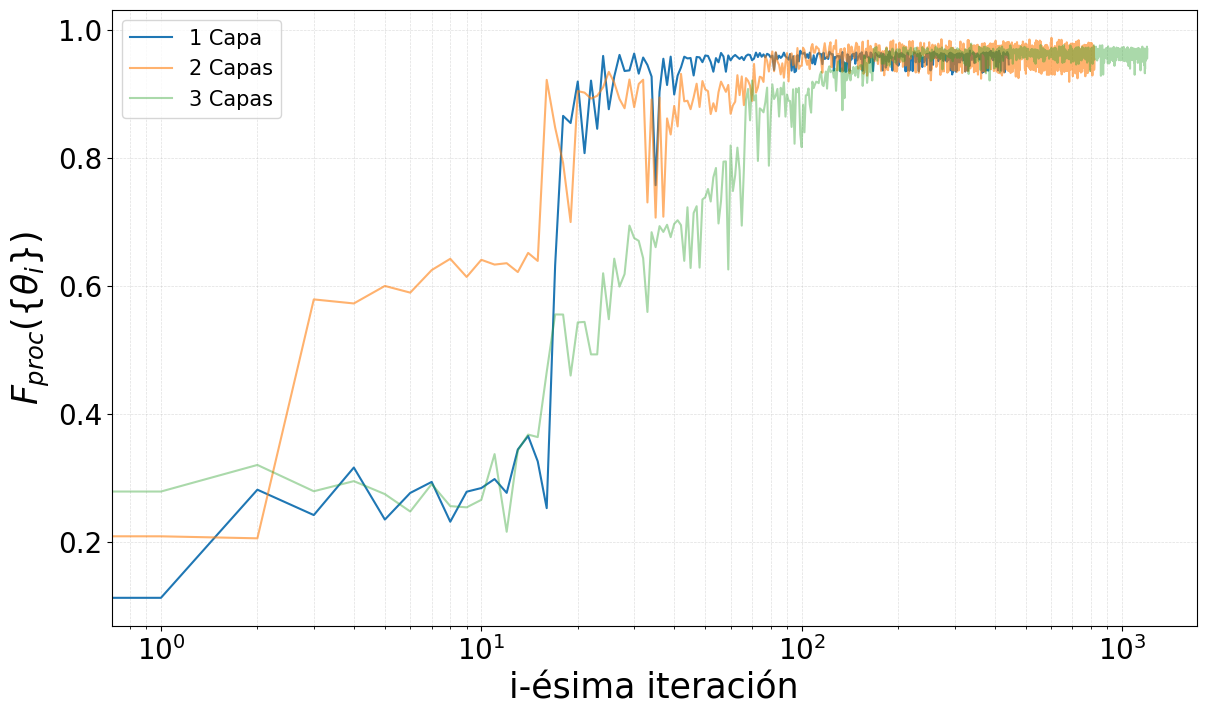
\includegraphics[width=0.70 \linewidth]{imagenes/comparacion_capas.png}
    \caption{Comparación de el proceso de optimización del ansatz utilizado
para el DP a diferentes capas. En azul vemos el resultado para una capa,
amarillo para dos y verde para tres. Estos resultados fueron ejecutados para un
valor de $p=0.125$. \textbf{Fuente}: elaboración propia.}
    \label{fig:comparacion_capas}
\end{figure} % }}}


Para la función \texttt{Minimize}() se fijaron dos hiper parámetros :
\texttt{method} y \texttt{tol}. Se utilizó el método \texttt{COBYLLA}, que
realiza la minimización mediante aproximaciones lineales, mientras que la
tolerancia se ajustó a $1\times 10^{-15}$. Se tomaron estos hiperparámetros
porque con ellos alcanzamos consistentemente la minimización de la función de
costo sin estresar de forma inecesaria el equipo de trabajo. 

Es importante mencionar las limitaciones al usar las computadoras cuánticas de
IBM, donde el tiempo de uso está limitado a 10 minutos mensuales\footnote{Este
es el tiempo de uso disponible en el plan gratuito de IBM.}. Vimos que el
tiempo de ejecución de una tomografía de proceso para un canal de un  qubit
requiere 12 circuitos, que lleva un tiempo de ejecución promedio de $16$s. Por
esta razón decidimos optimizar el \textit{ansatz} en el simulador cuántico y
posteriormente, ejecutar el circuito optimizado en una computadora cuántica.
Además, el simulador no tiene restricciones de tiempo, por ello ejecutamos el
\textit{ansatz} optimizado 4 veces para cada valor de $p$ en el simulador de
\texttt{AerSimualtor()}.

La función general se ejecutó para un listado de 38 valores distintos de $p$ en 
\texttt{p\_values}, ajustándose al tiempo mensual disponible en IBM, con un 
margen de error de una tomografía mensual. Cada circuito se ejecutó con 4000 
mediciones tanto en la computadora cuántica como en el simulador.  No incluimos 
todos los resultados detallados en esta sección para evitar sobrecargar la 
discusión\footnote{Se puede acceder al dataframe final, así como al código de 
este proyecto en el github: 
\href{https://github.com/felipechoy1/EPS/tree/main/Código\%20y\%20Resultados}{https://github.com/felipechoy1/EPS/tree/main/Código\%20y\%20Resultados}}.

Los resultados correspondientes a las fidelidades alcanzadas en la computadora
cuántica como en el simulador son presentadas en la figura
\ref{fig:comparacion_fidelidad}. Aquí obtenemos fidelidades en la computadora
cuántica en el rango de $0.553\leq F_{proc} \leq 0.974$. Por otro lado, para el
simulador, el promedio de las fidelidades en las 4 ejecuciones está en el rango
de $0.762\leq F_{proc} \leq 0.993$. Finalmente, al observar la desviación
estándar en los cálculos del simulador, se obtienen valores en el rango de
$0.001\leq \sigma_{F_{proc}} \leq 0.027$. Esta comparación se presenta en la
tabla \ref{tab:comparacion_fidelidades}.



\begin{figure}[h!] 
    \centering 
    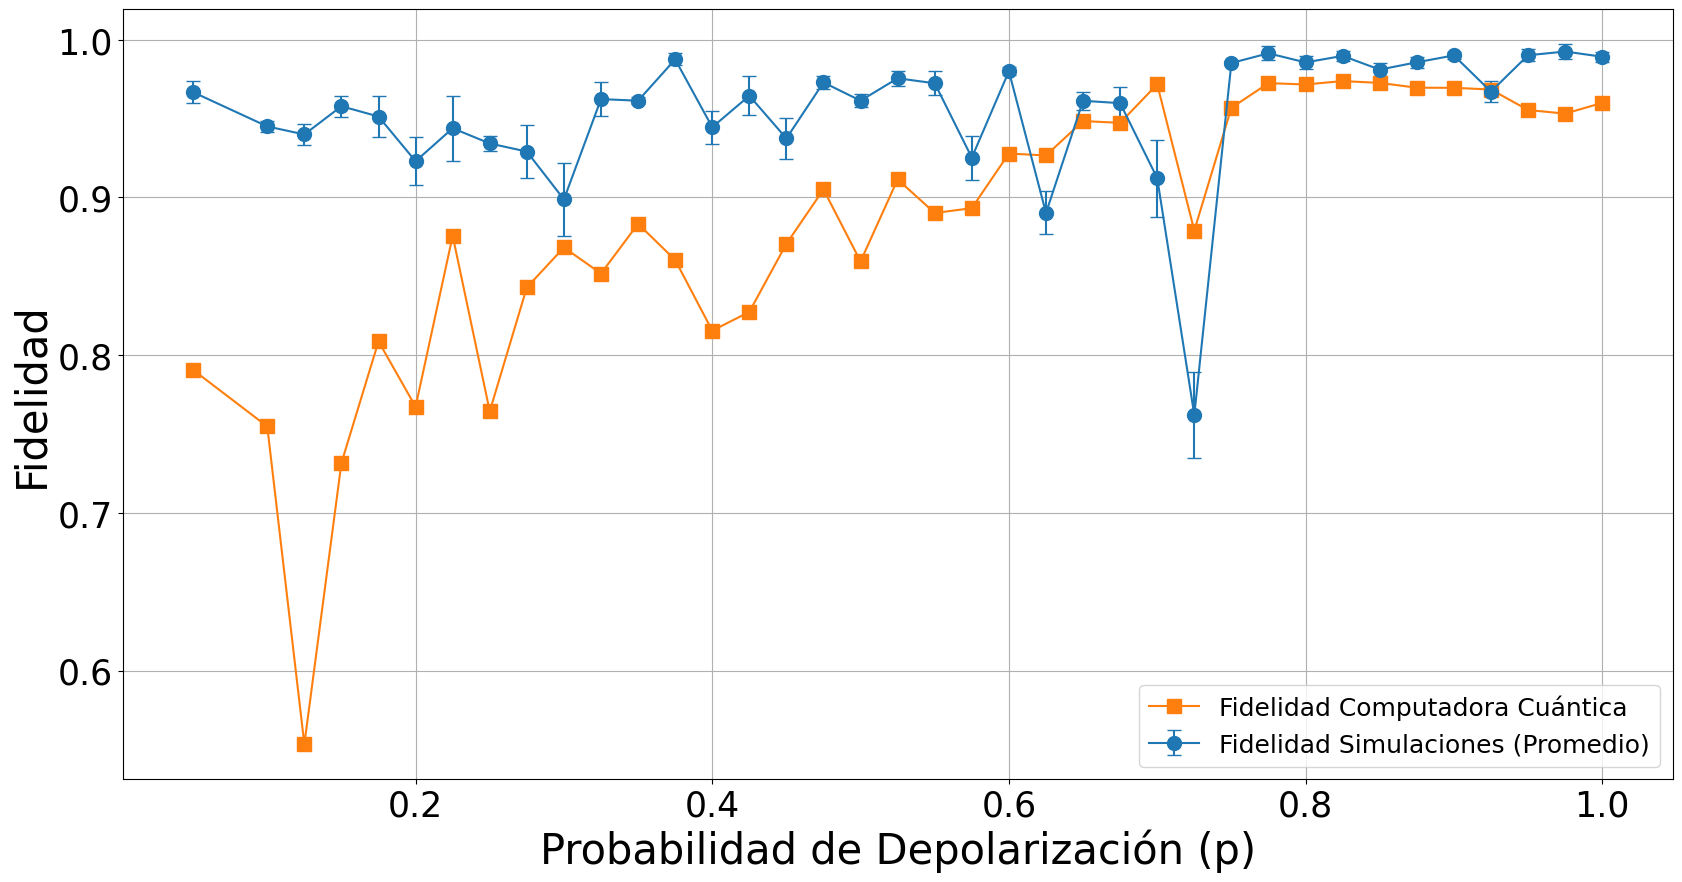
\includegraphics[width=0.7\linewidth]{imagenes/comparacion fidelidad.png}
    \caption{Comparación de fidelidades de proceso luego de ejecutar el \textit{ansatz}
optimizado. En azul se encuentra la fidelidad de la matriz de Choi reconstruida
en el simulador cuántico \texttt{AerSimualtor()}. Por otro lado en azul,
corresponde a la ejecución en la computadora cuántica \texttt{ibm-kyoto}.
\textbf{Fuente}: elaboración propia. }
    \label{fig:comparacion_fidelidad}
    \end{figure}
    

\begin{table}[htbp]
\centering 
\resizebox{\textwidth}{!}{
\begin{tabular}{|l|c|c|c|c|c|c|c|}
\hline
\textbf{Backend} & \textbf{Mediana} & \textbf{Mínimo} & \textbf{Máximo} & \textbf{p(max)} & \textbf{p(min)} & \textbf{Desv. Estándar} \\ \hline
Aer Simulator & 0.9618  & 0.7620  & 0.9925 & 0.975 & 0.725 & 0.0418 \\ \hline
ibm-kyoto     & 0.8916 & 0.5533 & 0.9738 & 0.825 & 0.125 & 0.0899  \\ \hline
\end{tabular}
}
\caption{Comparación de fidelidad de proceso entre las matrices de Choi
reconstruidas del \textit{ansatz} optimizado. Los resultados de la computadora cuántica
fueron tomados en \texttt{ibm-kyoto}, mientras que en el simulador fueron en
\texttt{AerSimualtor()} de Qiskit. \textbf{Fuente:} elaboración propia.}
\label{tab:comparacion_fidelidades}
\end{table}

Al mismo tiempo, evaluamos la completa positividad (CP) de las matrices de Choi reconstruidas por medio de sus autovalores. Para ello, sabemos que la matriz de Choi del DP esta dado por la ecuación \ref{ec:choi_depolarizing}, por lo que sus autovalores se calculan resolviendo la ecuación característica:
\begin{equation}
\det(\Lambda_\mathcal{E} - \lambda I) = 0,
\end{equation}
donde $\Lambda_\mathcal{E}$ es la matriz de Choi e $I$ es la matriz identidad
de dimensión $4 \times 4$. Para resolver esta ecuación, restamos $\lambda$ de
los elementos diagonales de $\Lambda_\mathcal{E}$:
\begin{equation}
\Lambda_\mathcal{E} - \lambda I = \begin{pmatrix}
1 - \frac{p}{2} - \lambda & 0 & 0 & 1 - p \\
0 & \frac{p}{2} - \lambda & 0 & 0 \\
0 & 0 & \frac{p}{2} - \lambda & 0 \\
1 - p & 0 & 0 & 1 - \frac{p}{2} - \lambda
\end{pmatrix}.
\end{equation}
Al encontrar la determinante de la matriz:
\begin{equation}
\left( \frac{p}{2} - \lambda \right)^2  \left[ \left( 1 - \frac{p}{2} - \lambda \right)^2 - (1 - p)^2 \right] = 0.
\end{equation}
Esto se puede factorizar como:
\begin{equation}
\left( \frac{p}{2} - \lambda \right)^2 \left( \lambda - \frac{p}{2} \right) \left( \lambda - \left( 2 - \frac{3p}{2} \right) \right) = 0.
\end{equation}
Por lo tanto, los autovalores de $\Lambda_{\mathcal{E}}$ son:
\begin{align}
\lambda_1 &=\lambda_2=\lambda_3 = \frac{p}{2} \quad \\
\lambda_4 &= 2 - \frac{3p}{2} .
\end{align}
Comparamos los autovalores de nuestros resultados en la figura
\ref{fig:comparacion_autovalores} para cada valor de $p$. Notamos que todos los
autovalores para todos los valores de $p$ cumplen con ser mayores o iguales a
0. Por lo tanto, los canales reconstruidos cumplen con ser CP.  Por otro
lado, al analizar la condición de preservación de la traza (TP) notamos que
ninguna de las matrices de Choi reconstruidas en ninguno de los sistemas cumple
con preservar la traza. Esto lo verificamos realizando la traza parcial de las matrices de Choi con \texttt{partial\_trace()}, obteniendo resultados que son cercanos a la matriz identidad $I$. Sin embargo, se observan valores no nulos en los elementos fuera de la diagonal, lo que impide que sean exactamente iguales a $I$ (ver figura \ref{fig:ident_comp}).
\begin{figure}[h!] 
    \centering 
    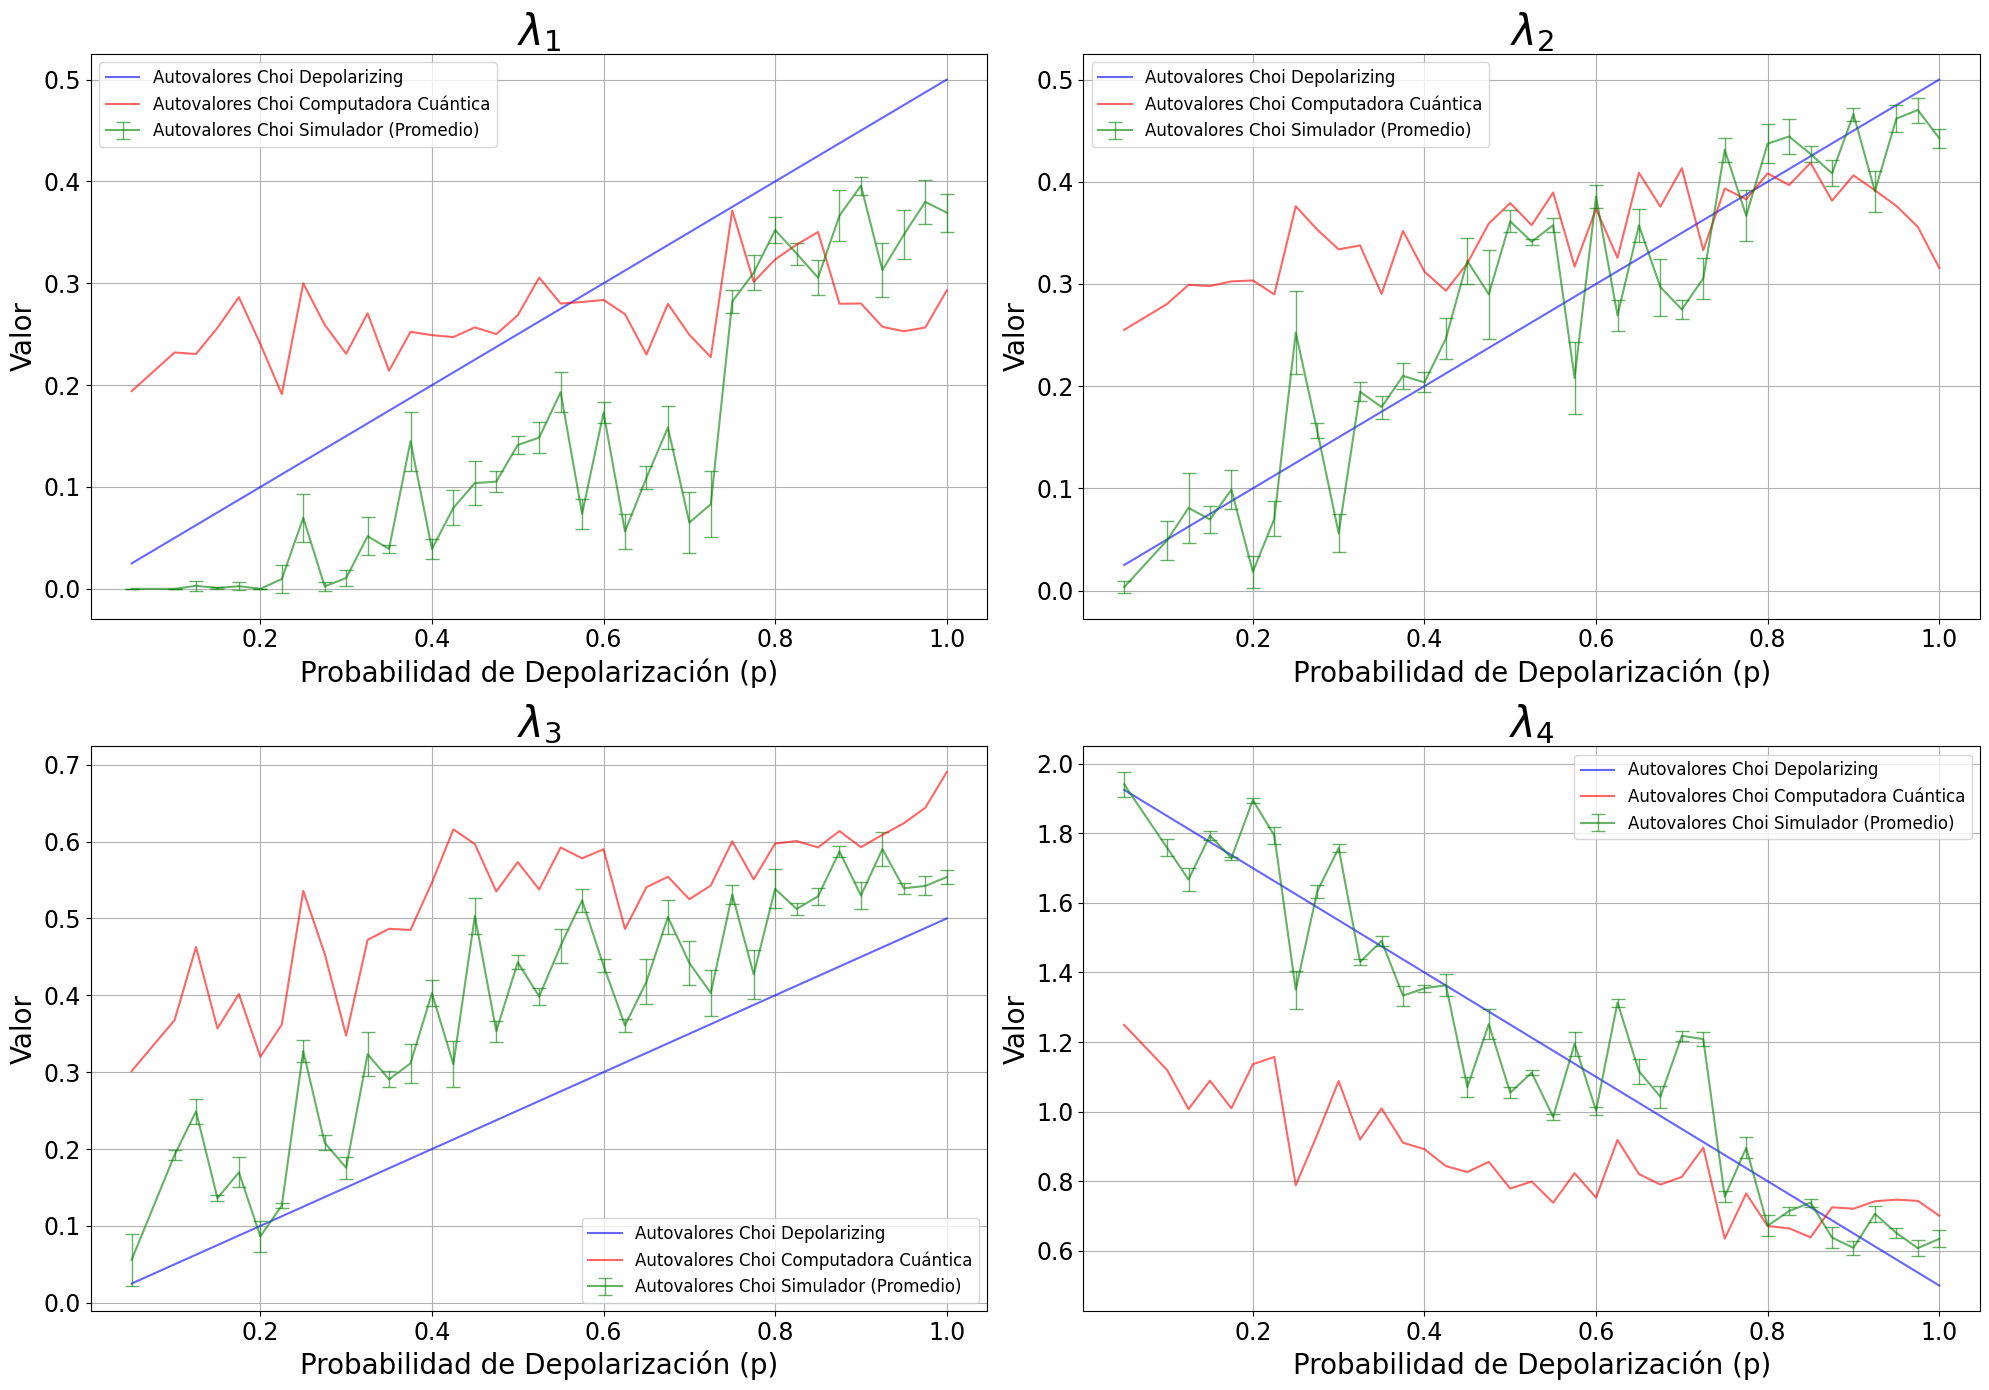
\includegraphics[width=0.90 \linewidth]{imagenes/eigenvalores_comparacion.png}
    \caption{Comparación de autovalores correspondientes a la matriz de Choi reconstruidas. En azul se puede ver el autovalor esperado a lo largo de $p$, en verde vemos el promedio de los valores de las matrices de Choi reconstruidas  en el simulador cuántico \texttt{AerSimualtor()}. Finalmente vemos en rojo los autovalores correspondientes a las matrices de Choi reconstruidas en la computadora cuántica \texttt{ibm-kyoto}. \textbf{Fuente}: elaboración propia. }
    \label{fig:comparacion_autovalores}
\end{figure}


\begin{figure}[h!] % {{{
    \centering
    % Subfigura para p = 0.1
    \begin{subfigure}{\textwidth}
        \centering
        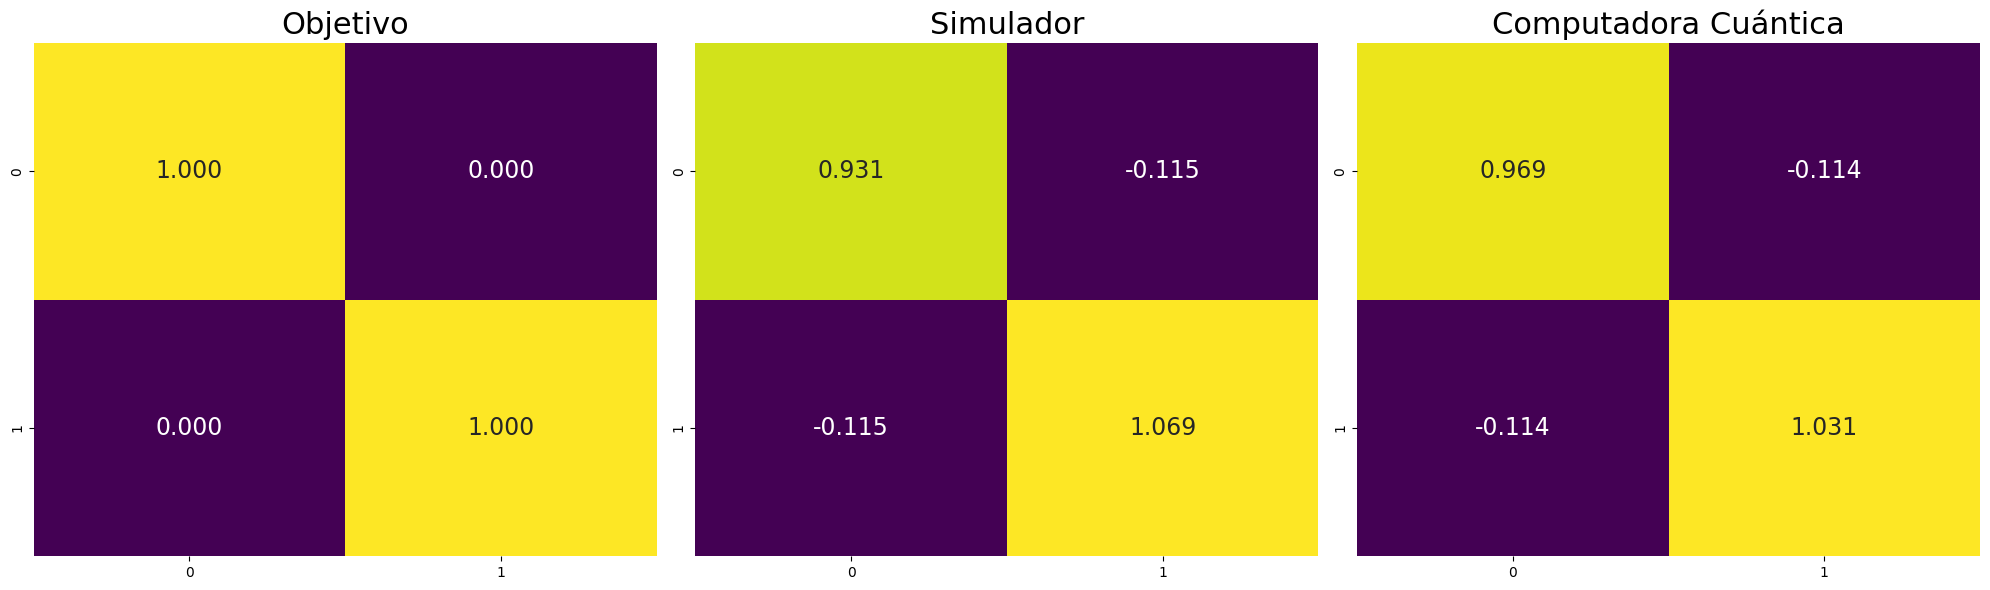
\includegraphics[width=0.9\linewidth]{imagenes/ident_comp_0.1.png}
        \caption{Comparación de matrices densidad reducidas para p = 0.1}
        \label{fig:ident_comp_p0.1}
    \end{subfigure}
    \vspace{1em} % Espacio vertical entre subfiguras
    
   
    % Subfigura para p = 0.9
    \begin{subfigure}{\textwidth}
        \centering
        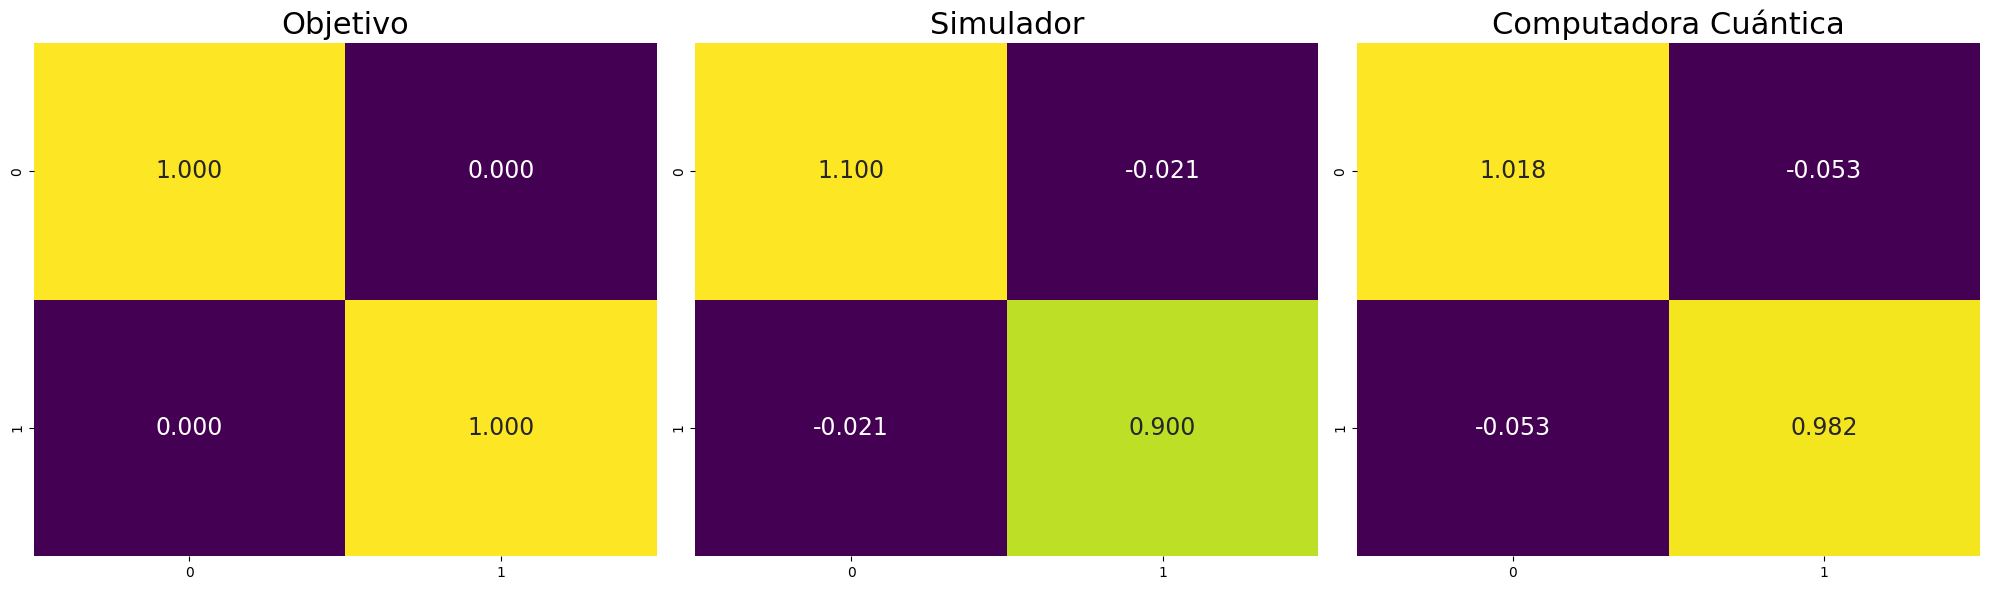
\includegraphics[width=0.9\linewidth]{imagenes/ident_comp_0.9.png}
        \caption{Comparación de matrices densidad reducidas para p = 0.9}
        \label{fig:ident_comp_p0.9}
    \end{subfigure}
 \caption{Comparación entre matrices de Choi reducidas objetivo  y  las matrices de Choi reducidas en el simulador cuántico \texttt{AerSimulator()}. Los valores se presentan para disntintas probabilidades de despolarización $p$ del DP. Cada valor representa una componente real de la matriz de Choi reducida. \textbf{Fuente:} elaboración propia.}
    \label{fig:ident_comp}
\end{figure}


% }}}
% }}}
\section{Discusión de Resultados} % {{{
En esta sección discutiremos sobre las diferencias encontradas entre las
fidelidades y autovalores calculados en el simulador y la computadora cuántica.
Vemos que estas diferencias se deben en gran parte a que la optimización fue
realizada en el simulador cuántico, el cual esta configurado en un entorno
ideal. 
% Vemos que estas diferencias se deben en gran parte a los errores inherentes al
% hardware cuántico real, como la decoherencia, errores en las compuertas
% cuánticas y limitaciones en la precisión de las mediciones. 


La figura \ref{fig:comparacion_fidelidad} así como la tabla
\ref{tab:comparacion_fidelidades} muestran que el simulador cuántico produce
resultados con fidelidades consistentemente cercanas a 1 a lo largo de todo el
rango de $p$. En contraste, la computadora cuántica presenta una mayor
variabilidad en sus resultados. Para analizar esta diferencia, realizamos una
regresión lineal de la fidelidad en función de $p$ tanto para la computadora
cuántica como para el simulador, como se muestra en la figura
\ref{fig:comparacion_regresiones}.

\begin{figure}[h!]
    \centering
    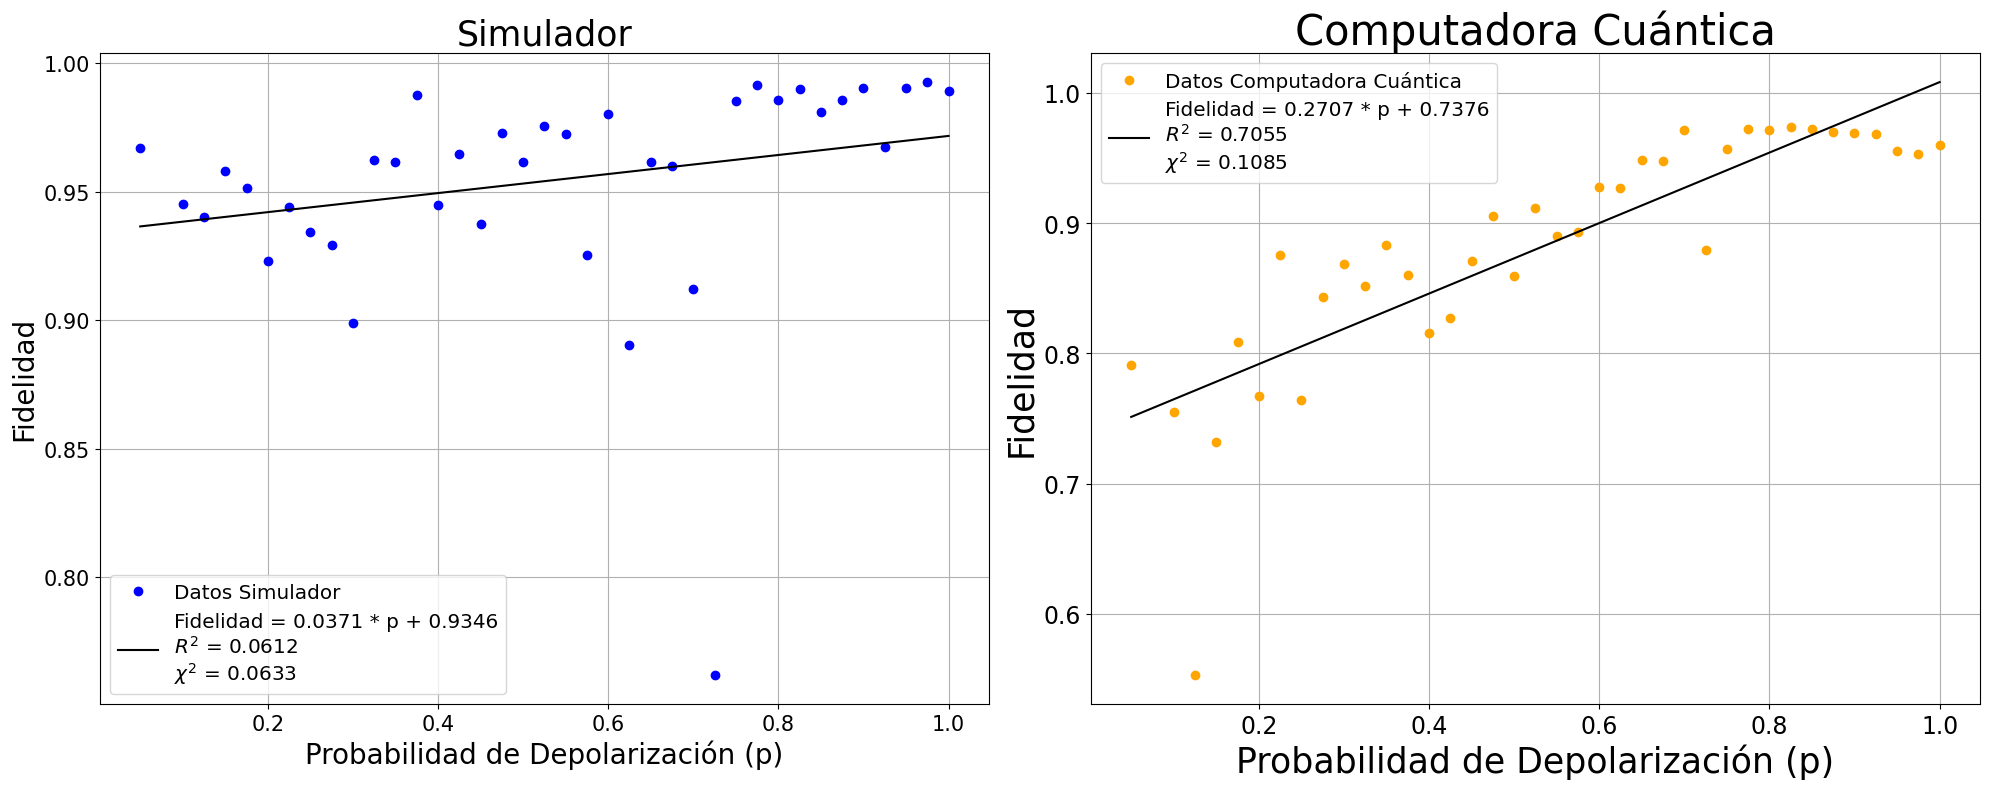
\includegraphics[width=0.95\linewidth]{imagenes/Comparacion_regresiones.png}
    \caption{Comparación de regresiones lineales entre los resultados de la fidelidad de proceso entre la matriz de Choi esperada , la computadora cuántica \texttt{ibm\_kyoto} y el simualdor cuántico \texttt{AerSimualtor()} respectivamente. \textbf{Fuente:} elaboración propia.}
    \label{fig:comparacion_regresiones}
\end{figure}

En el caso de la computadora cuántica, la ecuación de la regresión lineal es:
\begin{equation}
    F_{proc\_qc}(p) = 0.2707 \cdot p + 0.7376,
\end{equation}
con un coeficiente de determinación $R^2 = 0.7055$ y un valor de Chi-cuadrado
de $\chi^2 = 0.1085$.  Esto indica que la fidelidad tiende a aumentar con la
probabilidad de despolarización $p$, pero el ajuste no es perfecto. Los valores
de $R^2$ y $\chi^2$ sugieren que la relación no es estrictamente lineal y que
podría haber otros factores influyendo en los resultados en la computadora
cuántica. \felnote{También quisiera que hablaramos sobre las gráficas}. \cpnote{Va}

El aumento lineal de la fidelidad puede explicarse porque,
al aumentar $p$ en el DP, los estados se vuelven más
mixtos, reduciendo su sensibilidad a errores específicos del hardware cuántico.
En sistemas como \texttt{ibm\_kyoto}, una alta despolarización reduce la
sensibilidad del estado a errores de compuertas cuánticas y decoherencia, ya
que un estado menos puro tiende a ser menos afectado por estas imperfecciones.

Por otro lado, observamos que el simulador \texttt{AerSimulator()} tiene una
ecuación de la recta:
\begin{equation}
    F_{proc\_sim}(p) = 0.0371 \cdot p + 0.9346,
\end{equation}
con un coeficiente de determinación $R^2 = 0.0612$ y un valor de Chi-cuadrado
de $\chi^2 = 0.0633$. 
Aunque el bajo valor de $R^2$ indica que la relación entre la fidelidad y $p$
en el simulador es débil, sí se observa un aumento lineal sistemático en la
fidelidad con respecto a $p$. La pequeña pendiente de la recta sugiere que el
cambio en la fidelidad es leve y se mantiene prácticamente constante a lo largo
del rango de $p$, aunque no completamente insensible al aumento de $p$.

Analizamos la variabilidad de fidelidad en ambos casos, como se muestra en la
figura \ref{fig:comparacion_desviaciones}. En el simulador cuántico, no se
observa una tendencia clara en la desviación estándar de la fidelidad a lo
largo de $p$, excepto en el intervalo $0.6 \le p \leq 0.75$, que parece ser una
anomalía en los datos. Por otro lado, la computadora cuántica muestra una
reducción en la desviación estándar de la fidelidad a medida que aumenta $p$,
lo que confirma nuestra suposición basada en la regresión lineal. Finalmente,
en ambos casos, observamos que para valores de $p>0.75$, la desviación estándar
disminuye significativamente.\cpnote{Creo que hay varios estudios que sugieren que 
el comportamiento de la computadora cuántica de la IBM no es estacionario. 
Sería bueno citarlos. Hablemos también} \felnote{Pendiente: estuve investigando y me encontré con este paper: https://arxiv.org/pdf/2302.10881 . Aquí mencionan como los errores fuera de  resonancia pueden causar comporatmientos no estacionarios. Pero si quisiera que lo vieramos también.}


\begin{figure}[h!] % {{{
    \centering
    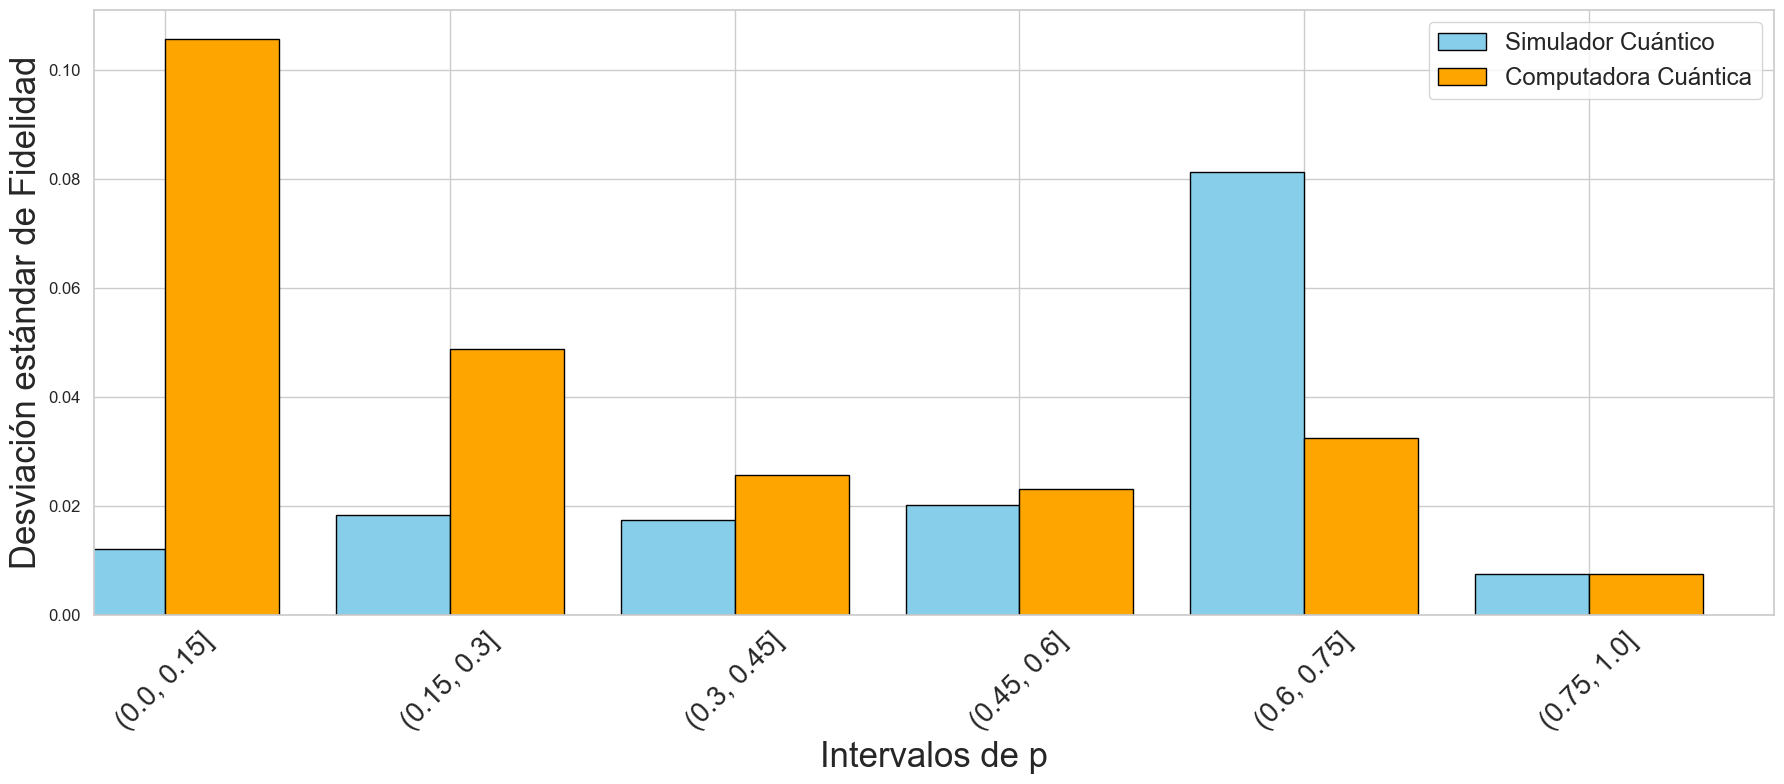
\includegraphics[width=0.95\linewidth]{imagenes/Comparacion_desviaciones.png}
    \caption{Comparación de desviación estándar entre los resultados de la fidelidad de proceso entre la matriz de Choi esperada , la computadora cuántica \texttt{ibm\_kyoto} (color naranja) y el simualdor cuántico (color azul) \texttt{AerSimualtor()}. La desviación estándar se calcula sobre los valores de fidelidad en el intervalo de $p$. \textbf{Fuente:} elaboración propia.}
    \label{fig:comparacion_desviaciones}
\end{figure} % }}}


Al analizar los cuatro autovalores presentados en la figura
\ref{fig:comparacion_autovalores}, notamos que tanto en el simulador como en la
computadora cuántica, los autovalores $\lambda_1,\lambda_2,\lambda_3$ no son
iguales entre sí. Además, en todos los casos, la computadora cuántica se desvía
más de los resultados esperados en comparación con el simulador.
Específicamente, observamos que la computadora cuántica comienza con valores
más altos para $\lambda_1,\lambda_2,\lambda_3$, y también con valores más bajos
para $\lambda_4$ en comparación con el simulador.  Estos primeros tres
autovalores están relacionados con la probabilidad de que el canal mantenga el
estado cuántico original, mientras que el cuarto autovalor corresponde a la
probabilidad de que el estado cuántico se vuelva completamente mixto. Por lo
tanto, estas observaciones sugieren que la computadora cuántica introduce más
ruido desde etapas tempranas, que se refleja en una tendencia menos pronunciada
en comparación con el simulador. Esta interpretación es coherente con los
resultados obtenidos en la regresión lineal, donde el intercepto de la
fidelidad en la computadora cuántica ($0.7376$) es menor que en el simulador,
que muestra fidelidades iniciales más altas y con menor variabilidad
($0.9346$).

En la figura \ref{fig:comparacion_choi}, observamos que las
matrices de Choi generadas por la computadora cuántica presentan mayor
coherencia en las entradas no diagonales. Esto también nos muestra que la
computadora cuántica introduce ruido desde un inicio del proceso de
despolarización debido a las imperfecciones inherentes al hardware y las
compuertas cuánticas. Notemos que al incrementar $p$, aumentamos la probabilidad de
despolarización, lo cual introduce más ruido a la interacción del sistema con
el estado máximamente mixto (ver ecuación
\ref{ec:superop_depolarizing}). Este proceso provoca una mejora en la
fidelidad porque, al hacer que los estados sean menos puros, se vuelven menos
sensibles a errores específicos del hardware cuántico. 

Por otro lado, las matrices obtenidas del simulador son
más consistentes con los valores teóricos, con valores casi nulos en las
posiciones no diagonales, reflejando mayor fidelidad en la simulación del canal
a lo largo de $p$.

\begin{figure}[h!] % {{{
    \centering
    % Subfigura para p = 0.1
    \begin{subfigure}{\textwidth}
        \centering
        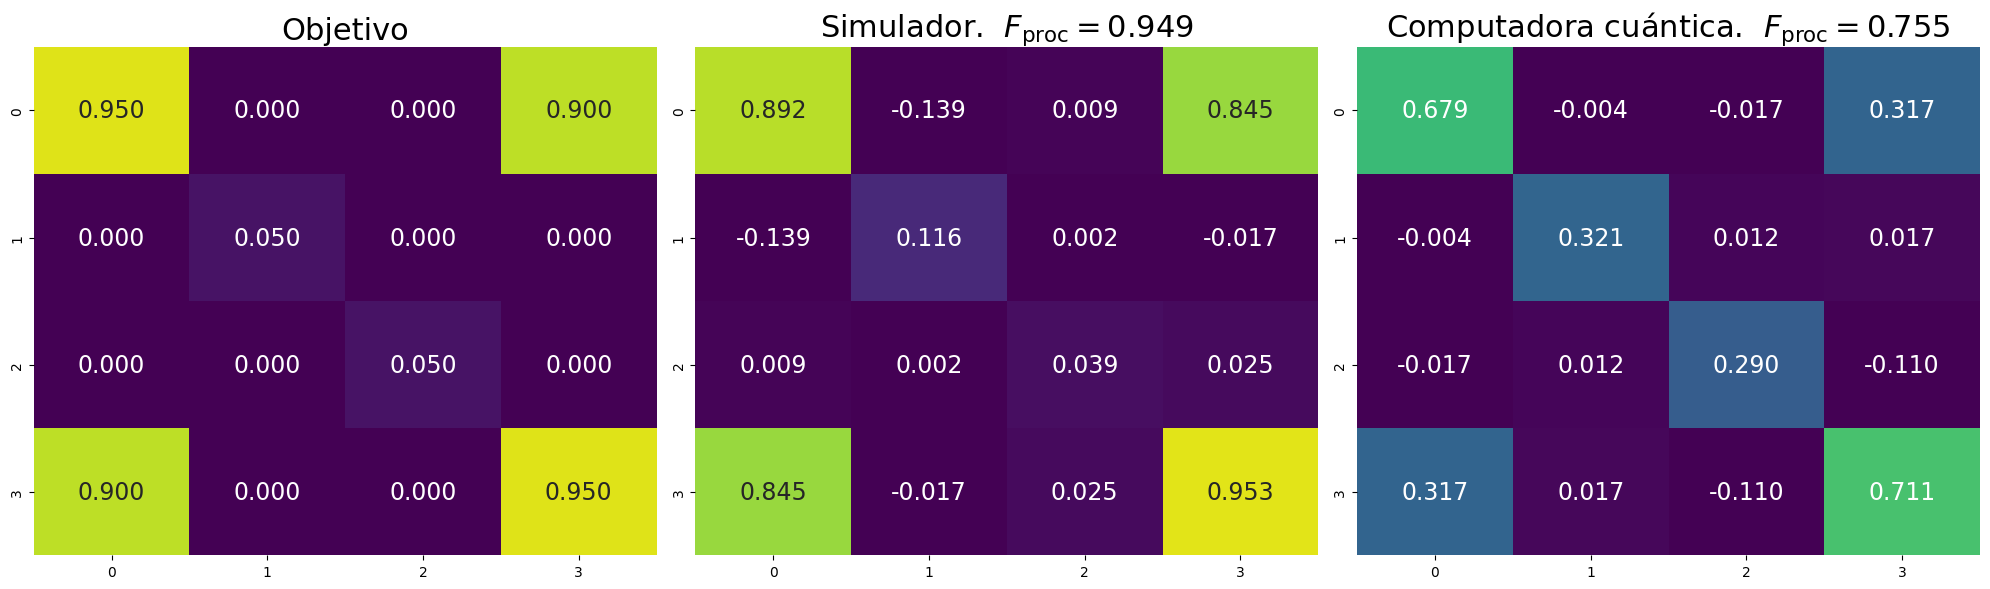
\includegraphics[width=1\linewidth]{imagenes/comp_choi_p0.1.png}
        \caption{Comparación de matrices de Choi para p = 0.1}
        \label{fig:choi_p0.1}
    \end{subfigure}
    \vspace{1em} % Espacio vertical entre subfiguras
    
    % Subfigura para p = 0.9
    \begin{subfigure}{\textwidth}
        \centering
        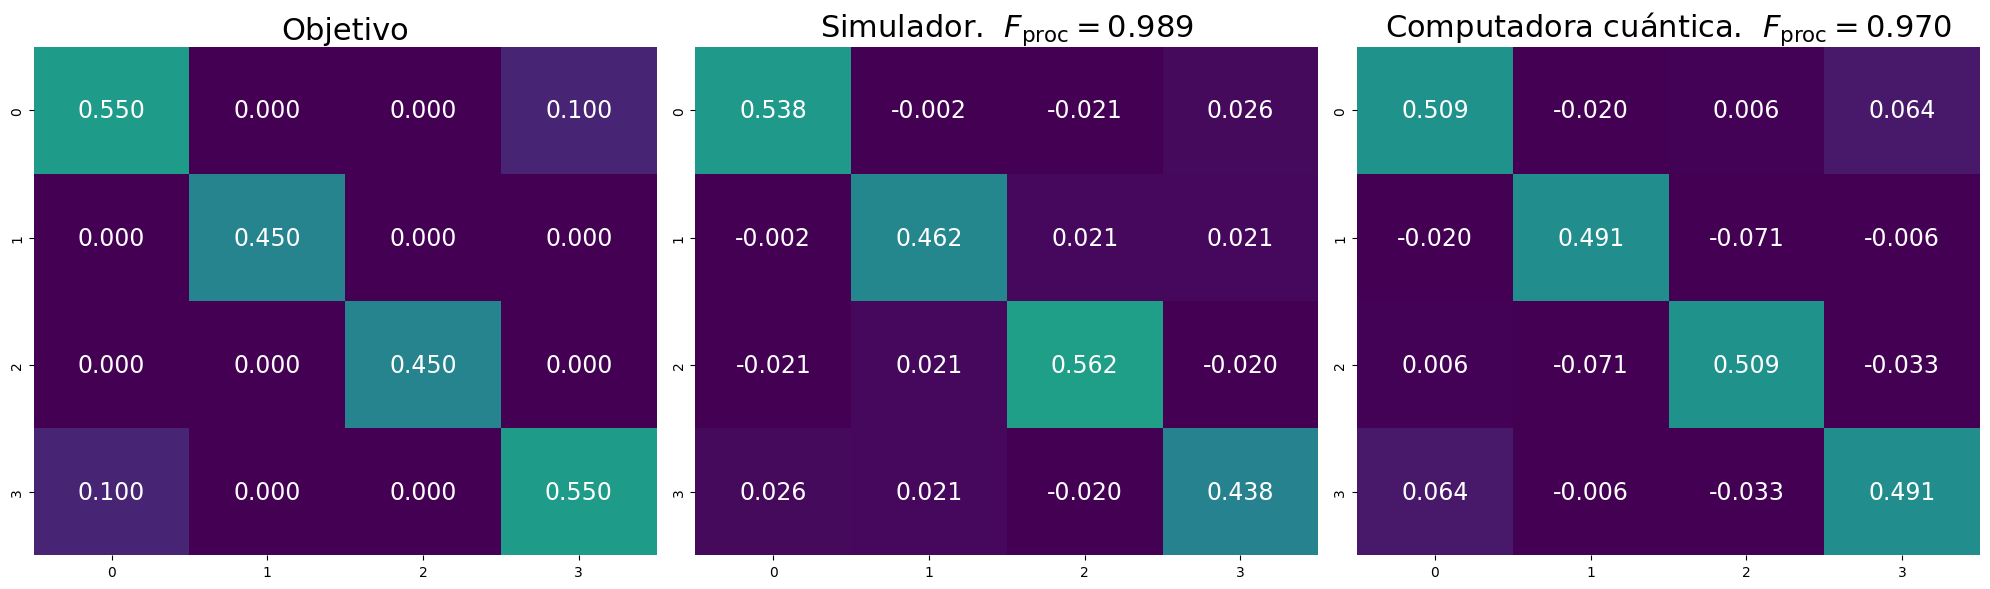
\includegraphics[width=1\linewidth]{imagenes/comp_choi_p0.9.png}
        \caption{Comparación de matrices de Choi para p = 0.9}
        \label{fig:choi_p0.9}
    \end{subfigure}
    
    \caption[Comparación de matrices de Choi objetivo y
reconstruidas]{
    Comparación de matrices de Choi objetivo y matrices de Choi reconstruidas en el simulador cuántico \texttt{AerSimulator()}, como en la computadora cuántica \texttt{ibm\_kyoto}. Los valores se presentan para disntintas probabilidades de despolarización $p$ del DP. Cada valor representa una componente real de la matriz de Choi. \textbf{Fuente:} elaboración propia.}
    \label{fig:comparacion_choi}
\end{figure} % }}

% }}}
% }}}
% }}}
\chapter{CONCLUSIONES} % {{{
\section{Conclusiones}
\section{Trabajo a Futuro}
\subsection{Implementación de VQA para 2 qubits}
% }}}
\appendix
% Notas sueltas {{{

% En la teoría cuántica, un sistema cuántico abierto es aquel que no está aislado, sino que interactúa continuamente con su entorno. Este tipo de sistemas son fundamentales para entender muchos fenómenos cuánticos en la práctica, ya que cualquier sistema cuántico real interactúa con su entorno. A diferencia de los sistemas cuánticos cerrados, que se consideran completamente aislados y evolucionan de manera unitaria según la ecuación de Schrödinger, los sistemas cuánticos abiertos pueden sufrir pérdidas de coherencia cuántica debido a estas interacciones. En la sección 3.1 exploraremos este tipo de sistemas por medio de canales cuánticos, con énfasis en su representación con la matriz de Choi. En la sección 3.2 mencionaremos la tomografía y fidelidad de proceso cuántico, ya que son importantes para la reconstrucción de canales cuánticos en computadoras cuánticas


% % Pendiente de redactar
% Los Algoritmos Variacionales Cuánticos (VQA) representan una estrategia innovadora en el campo de la computación cuántica para resolver problemas complejos. A través de un esquema híbrido que aprovecha tanto recursos cuánticos como clásicos, los VQA buscan optimizar un conjunto de parámetros en un circuito cuántico parametrizado. Estos algoritmos son fundamentales en tareas donde la solución se codifica dentro de una función de costo o pérdida, la cual es minimizada a través del ajuste variacional de parámetros dentro del circuito. \cite{VQA}

% El circuito cuántico parametrizado, o \textit{\textit}, es diseñado para ser versátil y adaptarse a la naturaleza del problema y las características del hardware cuántico disponible. Los \textit{ansatz} más efectivos, como el Hardware Efficient \textit{ansatz} (HEA), son aquellos que equilibran la expresividad del circuito y la eficiencia en términos de recursos y operaciones cuánticas requeridas. \cite{VQA}

% El proceso de optimización en VQAs se articula en tres fases principales:
% \begin{enumerate}
%     \item \textbf{Inicialización:} Se comienza con la preparación de un estado cuántico de referencia, sobre el cual se aplicarán las operaciones del \textit{\textit{ansatz}}.
%     \item \textbf{Aplicación del \textit{ansatz}:} Se utiliza el \textit{\textit{ansatz}} para transformar el estado inicial en un estado final que depende de los parámetros variacionales. Este paso es crítico y requiere una cuidadosa selección y configuración de las puertas cuánticas para navegar el espacio de Hilbert eficazmente.
%     \item \textbf{Evaluación y Optimización:} Se evalúa la función de costo mediante mediciones cuánticas y se emplea un optimizador clásico para ajustar los parámetros en busca de un mínimo, completando así el bucle cuántico-clásico.
% \end{enumerate}
% \subsubsection{Ejemplo: Inicialización de estados mixtos en computadoras cuánticas}
% Faltante de redactar




% \section{Aplicación de VQA para la simulación de Canales Cuánticos}
% Faltante de Redactar





% }}}
\bibliographystyle{abbrv}
\bibliography{references}   % Bibliografía
\end{document}
